% !Mode:: "Tex:UTF-8"









\documentclass[10pt,a4paper]{article}\usepackage[]{graphicx}\usepackage[]{color}
%% maxwidth is the original width if it is less than linewidth
%% otherwise use linewidth (to make sure the graphics do not exceed the margin)
\makeatletter
\def\maxwidth{ %
  \ifdim\Gin@nat@width>\linewidth
    \linewidth
  \else
    \Gin@nat@width
  \fi
}
\makeatother

\definecolor{fgcolor}{rgb}{0.345, 0.345, 0.345}
\newcommand{\hlnum}[1]{\textcolor[rgb]{0.686,0.059,0.569}{#1}}%
\newcommand{\hlstr}[1]{\textcolor[rgb]{0.192,0.494,0.8}{#1}}%
\newcommand{\hlcom}[1]{\textcolor[rgb]{0.678,0.584,0.686}{\textit{#1}}}%
\newcommand{\hlopt}[1]{\textcolor[rgb]{0,0,0}{#1}}%
\newcommand{\hlstd}[1]{\textcolor[rgb]{0.345,0.345,0.345}{#1}}%
\newcommand{\hlkwa}[1]{\textcolor[rgb]{0.161,0.373,0.58}{\textbf{#1}}}%
\newcommand{\hlkwb}[1]{\textcolor[rgb]{0.69,0.353,0.396}{#1}}%
\newcommand{\hlkwc}[1]{\textcolor[rgb]{0.333,0.667,0.333}{#1}}%
\newcommand{\hlkwd}[1]{\textcolor[rgb]{0.737,0.353,0.396}{\textbf{#1}}}%

\usepackage{framed}
\makeatletter
\newenvironment{kframe}{%
 \def\at@end@of@kframe{}%
 \ifinner\ifhmode%
  \def\at@end@of@kframe{\end{minipage}}%
  \begin{minipage}{\columnwidth}%
 \fi\fi%
 \def\FrameCommand##1{\hskip\@totalleftmargin \hskip-\fboxsep
 \colorbox{shadecolor}{##1}\hskip-\fboxsep
     % There is no \\@totalrightmargin, so:
     \hskip-\linewidth \hskip-\@totalleftmargin \hskip\columnwidth}%
 \MakeFramed {\advance\hsize-\width
   \@totalleftmargin\z@ \linewidth\hsize
   \@setminipage}}%
 {\par\unskip\endMakeFramed%
 \at@end@of@kframe}
\makeatother

\definecolor{shadecolor}{rgb}{.97, .97, .97}
\definecolor{messagecolor}{rgb}{0, 0, 0}
\definecolor{warningcolor}{rgb}{1, 0, 1}
\definecolor{errorcolor}{rgb}{1, 0, 0}
\newenvironment{knitrout}{}{} % an empty environment to be redefined in TeX

\usepackage{alltt}
\usepackage{etoolbox}
\newtoggle{color}
%\togglefalse{color}
\toggletrue{color}

\usepackage{makeidx}
\newcommand{\idioma}{spanish}
\newcommand{\opcionesIdioma}{,es-nodecimaldot,es-tabla}
% !Mode:: "Tex:UTF-8"
%%%%%%%%%%%%%%%%%%%%%Carga de Packages
%%poner \newcommand{\idioma}{spanish} o \newcommand{\idioma}{english} en el documento
\usepackage{pdfsync}
\usepackage{srcltx}
\usepackage[\idioma\opcionesIdioma]{babel}
\usepackage[utf8x]{inputenc}
\usepackage[T1]{fontenc}
\usepackage{graphicx}
\graphicspath{{/users/fernando/figuras/}{./}{./figuras/}{/fernando/figuras/}{/fernando/figuras/jpg/}}
\usepackage{multicol}
\usepackage{epsfig}
%\usepackage{oberdiek}
\usepackage{listingsutf8}
\lstset{inputencoding=utf8/latin1}
%\lstset{extendedchars=true}
\lstset{ %
  language=R,                     % the language of the code
  basicstyle=\ttfamily\small,       % the size of the fonts that are used for the code
  numbers=left,                   % where to put the line-numbers
  numberstyle=\tiny\color{gray},  % the style that is used for the line-numbers
  stepnumber=1,                   % the step between two line-numbers. If it's 1, each line
                                  % will be numbered
  numbersep=5pt,                  % how far the line-numbers are from the code
  backgroundcolor=\color{white},  % choose the background color. You must add \usepackage{color}
  showspaces=false,               % show spaces adding particular underscores
  showstringspaces=false,         % underline spaces within strings
  showtabs=false,                 % show tabs within strings adding particular underscores
  frame=single,                   % adds a frame around the code
  rulecolor=\color{black},        % if not set, the frame-color may be changed on line-breaks within not-black text (e.g. commens (green here))
  tabsize=2,                      % sets default tabsize to 2 spaces
  %captionpos=,                   % sets the caption-position to bottom
  breaklines=true,                % sets automatic line breaking
  breakatwhitespace=false,        % sets if automatic breaks should only happen at whitespace
  %title=\lstname,                 % show the filename of files included with \lstinputlisting;
                                  % also try caption instead of title
  keywordstyle=\color{black},      % keyword style
  commentstyle=\color{Brown},   % comment style
  stringstyle=\color{black},      % string literal style
  escapeinside={\%*}{*)},         % if you want to add a comment within your code
  morekeywords={*,...},            % if you want to add more keywords to the set
  lineskip={-2.5pt} % single line spacing
}
%\usepackage{algorithm}
\usepackage{amsmath}
\usepackage{amsfonts}
\usepackage{amssymb}
\usepackage{amsthm}
\usepackage{fancybox}
\usepackage{fancyvrb}
\usepackage{rotating}
\usepackage{keystroke}
\usepackage{array}
\input{xy}
\xyoption{all}
%\usepackage[dvipsnames,usenames]{color}
\usepackage[usenames,dvipsnames,svgnames,table]{xcolor}
\usepackage{colortbl}
\usepackage{comment}
\excludecomment{spanish}
\excludecomment{english}
\includecomment{\idioma}

%\usepackage{noweb}
%\usepackage{clrscode}
\usepackage{eurosym}
\usepackage{wasysym}
\usepackage{multirow}
%\usepackage{margins}
\usepackage{lscape}
\usepackage{longtable}
\usepackage[normalem]{ulem}
\usepackage{xr-hyper}

%%NUEVO
\newcolumntype{C}{{\centering\arraybackslash}m{20mm}}
\newcommand{\centercell}[1]{\multicolumn{1}{c}{#1}}
\newcommand{\colHead}[1]{\centercell{\bfseries#1}}

\excludecomment{ocultar}


% Matriz (par‚ntesis)
\def\matr#1#2{\left(\begin{array}{#1}#2\end{array}\right)}
% Determinante (barras)
\def\deter#1#2{\left|\begin{array}{#1}#2\end{array}\right|}
% Sistema de ecuaciones. (llave a la izda.)
\def\seq#1#2{\left\{\begin{array}{#1}#2\end{array}\right.}
% Ecuaci\'on de varias lineas (sin llave a la izda.)
\def\evl#1#2{\begin{array}{#1}#2\end{array}}

%%%%%%%%%%%%%%%%%%%%%%%%%%%%%%%%%%%%%%%%%%%%%%
%%%%%%%%%%%%%%%%%%%%%%%%%%%%%%%%%%%%%%%%%%%%%%
%%%%%%%%%%%%%%%%% M\'{a}rgenes %%%%%%%%%%%%%%%%
%
%
%\parindent=0mm
%
%\textwidth=160mm
%\textheight=220mm
%\hoffset=-20mm
%\voffset=-15mm
%\parskip=0mm
\marginparsep=3mm
\marginparwidth=25mm
%
%%%%%%%%%%%%%%%%%%%%%%%%%%%% Contadores para listas de problemas
%\newcommand{\adc}{\addtocounter{enumi}{1}}
\newcommand{\adc}{\stepcounter{enumi}}
\newcommand{\adci}{\stepcounter{enumii}}
\newcommand{\xadc}{\addtocounter{xcounter}{1}}
\newcommand{\be}{\begin{enumerate}}
\newcommand{\ee}{\end{enumerate}}
\newcommand{\bi}{\begin{itemize}}
\newcommand{\ei}{\end{itemize}}
\newcounter{xcounter}


\newcommand{\nin}{{\noindent}}

%\newcounter{prob}{}
%\def\pr{\addtocounter{prob}{1}(\theprob)\ }
%\def\pr2{\addtocounter{prob}{2}(\theprob)\ }

%%%%%%%%%%%%%%%%%%%%%%%%%%%Fin de demostraciones, ejemplos, etc.
\newcommand{\fin}{$\square$}
%%%%%%%%%%%%%%%%%%%%%%%%%%Notaci\'{o}n matem\'{a}ticas generales
%\newcommand{\suc}[1]{\{#1_n\}}
%\newcommand{\sucn}[1]{\{#1_n\}_{n\in\mathbb{N}}}
%\newcommand{\ser}[1]{\sum #1_n}
%\newcommand{\sern}[1]{\sum_{n\geq 1} #1_n}
%\newcommand{\limn}{\lim_{n\rightarrow\infty}}
%\newcommand{\limnd}{\displaystyle\lim_{n\rightarrow\infty}}
%\newcommand{\mf}[1]{\mathbf{#1}}
%\newcommand{\mb}[1]{\mathbb{#1}}
%\newcommand{\D}[1]{\Dv_{\mf{#1}}}
%\newcommand{\bsigma}{\pmb{\sigma}}
%\newcommand{\bPhi}{\pmb{\Phi}}
%\newcommand{\vol}{\operatorname{vol}}
%\newcommand{\ldbr}{[\hspace{-1.5pt}[}
%\newcommand{\rdbr}{]\hspace{-1.5pt}]}
%\newcommand{\fpws}[2]{{#1}\ldbr{#2}\rdbr}
%\newcommand{\leftPui}{<\hspace{-3pt}<}
%\newcommand{\rightPui}{\hspace{-3pt}}
%\newcommand{\Pui}[2]{{#1}\hspace{-6pt}\leftPui{#2}\rightPui}
%\newcommand{\pdd}[2]{\dfrac{\partial{#1}}{\partial{#2}}}
%%%%%%%%%%Conjuntos de n\'{u}meros
\newcommand{\N}{\mathbb{N}} %conjunto de n\'{u}meros naturales
\newcommand{\Z}{\mathbb{Z}} %conjunto de n\'{u}meros enteros
\newcommand{\R}{\mathbb{R}} %conjunto de n\'{u}meros reales
\newcommand{\C}{\mathbb{C}} %conjunto de n\'{u}meros complejos
\newcommand{\Q}{\mathbb{Q}} %conjunto de n\'{u}meros racionales
\newcommand{\EP}{\mathbb{P}} %espacios proyectivos
\newcommand{\K}{\mathbb{K}} %cuerpo gen\'{e}rico
\newcommand{\A}{\mathbb{A}} %espacios afines

%%%%%%%%%%Estadistica
\newcommand{\MEAN}{\mathrm{E}}
\newcommand{\Var}{\mathrm{Var}}
\newcommand{\Cov}{\mathrm{Cov}}


%%%%%%%%%%Funciones
\def\arcsen{\operatorname{arcsen}}
\def\arctg{\operatorname{arctg}}
\def\argCosh{\operatorname{argCosh}}
\def\argSenh{\operatorname{argSenh}}
\def\argTgh{\operatorname{argTgh}}
\def\cosec{\operatorname{cosec}}
\def\Cosh{\operatorname{Cosh}}
\def\cotg{\operatorname{cotg}}
\def\Dv{\operatorname{D}}
\def\discrim{\operatorname{discrim}}
\def\dive{\operatorname{div}}
\def\dom{\operatorname{dom}}
\def\Ext{\operatorname{Ext}}
\def\Fr{\operatorname{Fr}}
\def\dder#1#2{\dfrac{d #1}{d #2} } %derivada en estilo display
\def\gr{\operatorname{gr}}
\def\grad{\operatorname{grad}}
\def\Imag{\operatorname{Im}}
\def\mcm{\operatorname{mcm}}
\def\rang{\operatorname{rang}}
\def\rot{\operatorname{rot}}
\def\sen{\operatorname{sen}}
\def\Senh{\operatorname{Senh}}
\def\sgn{\operatorname{sgn}}
\def\sig{\operatorname{sig}}
\def\tg{\operatorname{tg}}
\def\Tgh{\operatorname{Tgh}}
\def\E{\operatorname{E}}
\def\VAR{\operatorname{VAR}}
\newcommand{\margWeb}[2]{\noindent{#2}\marginpar[\hspace{-18mm}\link{#1}{WEB}]{\hspace*{-18mm}\link{#1}{WEB}}}

%%%%%%%%%%%%%%%%%%%%%%\'{A}lgebra conmutativa.
\def\multideg{\operatorname{multideg}} %multidegree of a polynomial
\def\LT{\operatorname{lt}} %leading term of a polynomial
\def\LC{\operatorname{lc}} %leading coefficient of a polynomial
\def\LM{\operatorname{lm}} %leading monomial of a polynomial
\def\Mexp{\mathbb{Z}^n_{\geq 0}} %set of multiexponents of monomials
\def\set#1{\left\{{#1}\right\}}
\newcommand{\vlist}[2]{\mbox{${#1}_{1},\ldots,{#1}_{#2}$}}
\def\deg{\operatorname{deg}} %grado de un polinomio
\def\cp{\operatorname{cp}} %coeficiente principal de un polinomio
\def\CP{\operatorname{cp}} %coeficiente principal de un polinomio
\def\set#1{\left\{{#1}\right\}} %llaves de conjunto
\newcommand{\V}{{\bf V}} %variedad de un conjunto de polinomios
\newcommand{\I}{{\bf I}} %ideal de un conjunto
\newcommand{\MCD}{\operatorname{mcd}} %m\'{a}ximo com\'{u}n divisor
\newcommand{\MCM}{\operatorname{mcm}} %m\'{\i}nimo com\'{u}n m\'{u}ltiplo
\newcommand{\LCM}{\operatorname{lcm}} %least common multiple
\newcommand{\GCD}{\operatorname{gcd}} %greatest common divisor
\newcommand{\Ker}{\operatorname{Ker}} %N\'{u}cleo
\newcommand{\IM}{\operatorname{IM}} %Imagen
\newcommand{\Rad}{\operatorname{Rad}} %radical de un ideal
\newcommand{\Jac}{\operatorname{Jac}} %radical de Jacobson de un anillo
\newcommand{\Ann}{\operatorname{Ann}} %anulador de un ideal
\newcommand{\Res}{\operatorname{Res}} %resultante de polinomios
\newcommand{\Mult}{\operatorname{mult}} %multiplicidad
\newcommand{\Gen}{\operatorname{Gen}} %g\'{e}nero
\newcommand{\Card}{\operatorname{Card}} %cardinal
\newcommand{\ord}{\operatorname{ord}} %orden
\newcommand{\prim}{\operatorname{prim}} %parte primitiva
\newcommand{\NP}{\operatorname{NP}} %NP idea
\newcommand{\cont}{\operatorname{cont}} %parte primitva
\newcommand{\pp}{\operatorname{pp}} %parte primitva
\newcommand{\PP}{\mathop{\mathrm{PP}}\nolimits}
\newcommand{\Int}{\operatorname{Int}}
\newcommand{\Ind}{\operatorname{index}}
\newcommand{\Lcoeff}{\operatorname{lc}} %leading coefficient of a polynomial
\newcommand{\Sqf}{\operatorname{Sqf}} %square free part of a polynomial

\def\pd#1#2{\frac{\partial #1}{\partial #2}} %derivada parcial
\def\mult{\text{mult}} %multiplicity
\def\Sing{\text{Sing}} %multiplicity
\def\Cl#1{\overline{#1}} %cierre topol\'{o}gico
\def\fobox#1{\begin{center}\fbox{$\displaystyle #1 $}\end{center}}

%\newcommand{\Ext}{\operatorname{Ext}}

%%%%%%%%%%%%%%%%%%%%%%%%
%% unpunto mayor que cdot, pero menor que bullet
\newcommand{\sbt}{\,\begin{picture}(-1,1)(-1,-3)\circle*{3}\end{picture}\ }

%%%%%%%%%%%%%%%%%%%%%%%%S\'{\i}mbolos rodeados de un c\'{\i}rculo
\def\circled#1{\xymatrix{*+[o][F]{#1}}}

%%%%%%%%%%%%%%%%%%%Geometr\'{\i}a
\newcommand{\CH}{{\cal CH}} %%cierre convexo

%%%%%%%%%%%%%%%%%%%%Tipos de letra especiales
%%Caligr\'{a}ficas
\newcommand{\cA}{{\cal A}}
\newcommand{\cB}{{\cal B}}
\newcommand{\cC}{{\cal C}}
\newcommand{\cD}{{\cal D}}
\newcommand{\cE}{{\cal E}}
\newcommand{\cF}{{\cal F}}
\newcommand{\cG}{{\cal G}}
\newcommand{\cH}{{\cal H}}
\newcommand{\cI}{{\cal I}}
\newcommand{\cJ}{{\cal J}}
\newcommand{\cK}{{\cal K}}
\newcommand{\cL}{{\cal L}}
\newcommand{\cM}{{\cal M}}
\newcommand{\cN}{{\cal N}}
\newcommand{\cO}{{\cal O}}
\newcommand{\cP}{{\cal P}}
\newcommand{\cQ}{{\cal Q}}
\newcommand{\cR}{{\cal R}}
\newcommand{\cS}{{\cal S}}
\newcommand{\cT}{{\cal T}}
\newcommand{\cU}{{\cal U}}
\newcommand{\cV}{{\cal V}}
\newcommand{\cW}{{\cal W}}
\newcommand{\cX}{{\cal X}}
\newcommand{\cY}{{\cal Y}}
\newcommand{\cZ}{{\cal Z}}

%%%%%%%%%%%%%%%%%%%%%%%%%%Notaci\'{o}n matem\'{a}ticas generales
\newcommand{\sucn}[1]{\{#1_n\}_{n\in\mathbb{N}}}
\newcommand{\ser}[1]{\sum #1_n}
\newcommand{\sern}[1]{\sum_{n\geq 1} #1_n}
\newcommand{\limn}{\lim_{n\rightarrow\infty}}
\newcommand{\mf}[1]{\mathbf{#1}}
\newcommand{\mb}[1]{\mathbb{#1}}
\newcommand{\D}[1]{\Dv_{\mf{#1}}}
\newcommand{\bsigma}{\pmb{\sigma}}
\newcommand{\bPhi}{\pmb{\Phi}}
\newcommand{\vol}{\operatorname{vol}}
\newcommand{\ldbr}{[\hspace{-1.5pt}[}
\newcommand{\rdbr}{]\hspace{-1.5pt}]}
\newcommand{\fpws}[2]{{#1}\ldbr{#2}\rdbr}
\newcommand{\leftPui}{<\hspace{-3pt}<}
\newcommand{\rightPui}{\hspace{-3pt}}
\newcommand{\Pui}[2]{{#1}\hspace{-6pt}\leftPui{#2}\rightPui}
\newcommand{\pdd}[2]{\dfrac{\partial{#1}}{\partial{#2}}}


%\newcounter{contEnlace}

%\newcommand{\pendiente}{\textcolor{purple}{PENDIENTE: }}
%\newcommand{\link}[2]{\textcolor{blue}{{\href{#1}{#2}}}}


\iftoggle{color}{%
  % color version
  \newcommand{\pendiente}{\textcolor{red}{PENDIENTE: }}
  \newcommand{\link}[2]{\textcolor{blue}{{\href{#1}{#2}}}}
  \newcommand{\fichero}[2]{\textattachfile{#1}{\textcolor{blue}{#2}}}
  \newcommand{\otrofichero}[2]{\textattachfile{./datos/#1}{\textcolor{blue}{#2}}}
}{%
  % b/w version
  \newcommand{\pendiente}{\textcolor{black}{\underline{PENDIENTE:} }}
  \newcommand{\link}[2]{\textcolor{black}{{\href{#1}{\underline{#2}}}}}
  \newcommand{\fichero}[2]{\textattachfile{#1}{\textcolor{black}{\underline{#2}}}}
  \newcommand{\otrofichero}[2]{\textattachfile{./datos/#1}{\textcolor{black}{\underline{#2}}}}
}



%{\textcolor{blue}{{\href{#1}{#2}}}}

%%%%%%%%%%%%%%%%%%COLORES

\DefineNamedColor{named}{Brown}{cmyk}{0,0.81,1,0.60}
\definecolor{Gris050}{gray}{0.50}
\definecolor{Gris025}{gray}{0.75}
\definecolor{Gris010}{gray}{0.90}


%%%%%%%%%%%%%%%%%%%%%Package Algorithms
%\begin{spanish}
%\renewcommand{\algorithmicrequire}{{precondici\'{o}n:}}
%\renewcommand{\algorithmicensure}{{postcondici\'{o}n:}}
%\renewcommand{\algorithmicend}{{fin}}
%\renewcommand{\algorithmicif}{{si}}
% \renewcommand{\algorithmicthen}{{entonces}}
% \renewcommand{\algorithmicelse}{{si no}}
% \renewcommand{\algorithmicelsif}{\algorithmicelse\ \algorithmicif}
% \renewcommand{\algorithmicendif}{\algorithmicend\ \algorithmicif}
% \renewcommand{\algorithmicfor}{{para}}
% \renewcommand{\algorithmicforall}{{para todo}}
% \renewcommand{\algorithmicdo}{{hacer}}
% \renewcommand{\algorithmicendfor}{\algorithmicend\ \algorithmicfor}
% \renewcommand{\algorithmicwhile}{{mientras}}
% \renewcommand{\algorithmicendwhile}{\algorithmicend\ \algorithmicwhile}
% \renewcommand{\algorithmicrepeat}{{repetir}}
% \renewcommand{\algorithmicuntil}{{hasta}}
% \end{spanish}

%%%%%%%%%%%%%%%%%%%%%%%%%%%%%%%%%%Package Amsthm
\begin{spanish}
%\theoremstyle{definition}% default
\theoremstyle{plain}
\newtheorem{thm}{Teorema}[section]
\newtheorem{teo}{Teorema}[section]
\newtheorem{teorema}{Teorema}[section]
\newtheorem{lem}[thm]{Lema}
\newtheorem{lema}[thm]{Lema}
\newtheorem{prop}[thm]{Proposici\'{o}n}
\newtheorem{proposicion}[thm]{Proposici\'{o}n}
\newtheorem{cor}[thm]{Corolario}
\newtheorem{corolario}[thm]{Corolario}
\newtheorem*{KL}{Klein's Lemma}
%\theoremstyle{definition}
\newtheorem{defn}[thm]{Definici\'{o}n}
\newtheorem{definicion}[thm]{Definici\'{o}n}
\newtheorem{conj}[thm]{Conjetura}
\newtheorem{conjetura}[thm]{Conjetura}
\newtheorem{definicionInformal}[thm]{Definición Informal}
\newtheorem{exmp}[thm]{Ejemplo}
\newtheorem{ejemplo}[thm]{Ejemplo}
\newtheorem{Ejemplo}[thm]{Ejemplo}
\newtheorem{ejem}[thm]{Ejemplo}
\newtheorem{ejercicio}{Ejercicio}
%\theoremstyle{remark}
\newtheorem*{rem}{Observaci\'{o}n}
\newtheorem{observacion}[thm]{Observaci\'{o}n}
\newtheorem*{note}{Nota}
\newtheorem{nota}[thm]{Nota}
\newtheorem{case}[thm]{Caso}
\newtheorem{caso}[thm]{Caso}
\newtheorem{regla}[thm]{Regla}

\theoremstyle{remark}
\newtheorem{enlace}{$\bullet$ }
\end{spanish}

\begin{english}
\theoremstyle{plain}% default
%\theoremstyle{definition}
\newtheorem{thm}{Theorem}[section]
\newtheorem{lem}[thm]{Lemma}
\newtheorem{prop}[thm]{Proposition}
\newtheorem{cor}[thm]{Corollary}
\newtheorem*{KL}{Klein's Lemma}
\newtheorem{defn}[thm]{Definition}
\newtheorem{conj}[thm]{Conjecture}
\newtheorem{exmp}[thm]{Example}
\theoremstyle{remark}
\newtheorem*{rem}{Remark}
\newtheorem*{note}{Note}
\newtheorem{case}{Case}
\end{english}

%%%%%%%%%%%%%%%Package Listings
%\lstset{showstringspaces=false}
%\newcommand{\PAS}[1]{\lstinline@#1@}
%\newcommand{\CPP}[1]{\lstinline@#1@}


%%%%%%%%%%%%Estilo para bibliograf\'{\i}a

%\bibliographystyle{plain}

%%%%%%%%%%%%Mis anotaciones
\newcommand{\Pendiente}[1]{\textcolor{red}{Pendiente: #1}}
%\newcommand{\Pendiente}{\textcolor{purple}{Pendiente: }}

\newcommand{\fernando}[1]{\textcolor{red}{Fernando: #1}}

%%%%%%%%%%%%%%%% Enlace al indice
%\renewcommand{\chaptermark}[1]{\markboth{\chaptername\ \thechapter.#1 \ref{index}}{}}

%%%%%%%%%%%%%%%%%%Traducci\'{o}n de clrscode
%\renewcommand{\For}{\textbf{Para} }
%\renewcommand{\To}{\textbf{hasta} }
%\renewcommand{\By}{\textbf{incremento} }
%\renewcommand{\Downto}{\textbf{downto} }
%\renewcommand{\While}{\textbf{mientras} }
%\renewcommand{\Repeat}{\textbf{repetir}\\\addtocounter{indent}{1}}
%\renewcommand{\Until}{\kill\addtocounter{indent}{-1}\liprint\\\textbf{hasta que}\hspace*{-0.7em}\'}
%\renewcommand{\If}{\textbf{si} }
%\renewcommand{\Then}{\\textbf{entonces}\hspace{13mm}\\addtocounter{indent}{1}}
%\renewcommand{\Else}{\kill\addtocounter{indent}{-1}\liprint\\textbf{sino}\\addtocounter{indent}{1}}
%\renewcommand{\End}{\addtocounter{indent}{-1}}
%\renewcommand{\ElseIf}{\kill\addtocounter{indent}{-1}\liprint\textbf{sino si} }
%\renewcommand{\ElseNoIf}{\kill\addtocounter{indent}{-1}\liprint\textbf{si no}\addtocounter{indent}{1}}
%\renewcommand{\Do}{\\\textbf{hacer}\hspace*{-0.7em}\'\addtocounter{indent}{1}}
%\renewcommand{\Return}{\textbf{devolver} }
%\renewcommand{\Comment}{$\hspace*{-0.075em}\rhd$ }
%\renewcommand{\RComment}{\`\Comment}
%\renewcommand{\Goto}{\textbf{Ir a} }
%\renewcommand{\Error}{\textbf{error} }


%%%%%%%%%%%%%%%%%%%%%%%%%%%%%%%%%%%%%%%%%%%%%%%%%%%%%%%%%%%%%%%
%Cabecera para ejercicios
%\documentclass[11pt]{article}
%\newcommand{\idioma}{spanish}
%\input definiciones
%
%\textwidth=160mm \textheight=240mm \hoffset=-20mm \voffset=-30mm
%%\parskip=0mm
%%\marginparsep=-25mm \evensidemargin=82pt\evensidemargin=44pt
%
%
%\includecomment{solucion}
%%\excludecomment{solucion}

%%Compatibilidad con documentos antiguos
\newcounter{prob}{}
\def\pr{\noindent\addtocounter{prob}{1}(\theprob)\ }
\def\bepro{ \setcounter{prob}{0}}

%%Compatibilidad con documentos antiguos
% \def\ojo#1{
% \noindent$\btr$#1
% \marginpar[
% {GeoGebra}]
% {GeoGebra}}

% \def\atencion#1{\noindent #1
% \marginpar[
% {\includegraphics*[scale=1,width=1.2cm,keepaspectratio=true]{./datos/hipoizda}}]
% {\includegraphics*[scale=1,width=1.2cm,keepaspectratio=true]{./datos/hipodcha}}}


\def\Rlogo#1{\noindent #1
\marginpar[
{\includegraphics*[scale=1,width=1.5cm,keepaspectratio=true]{./datos/Rlogo.jpg}}]
{\includegraphics*[scale=1,width=1.5cm,keepaspectratio=true]{./datos/Rlogo.jpg}}}

\def\calcLogo#1{#1}

%\def\calcLogo#1{\noindent #1
%\marginpar[
%{\includegraphics*[scale=1,width=1.2cm,keepaspectratio=true]{./datos/LogoHojaCalculo.png}}]
%{\includegraphics*[scale=1,width=1.2cm,keepaspectratio=true]{./datos/LogoHojaCalculo.png}}}


\def\ninja#1{\noindent #1
\marginpar[ {\includegraphics*[scale=1,width=1.2cm,keepaspectratio=true]{../fig/ninja_desk.png}}]
{\includegraphics*[scale=1,width=1.2cm,keepaspectratio=true]{../fig/ninja_desk.png}}}

\def\buda#1{\noindent #1
\marginpar[ {\includegraphics*[scale=1,width=1.2cm,keepaspectratio=true]{../fig/Computer-Buddha.png}}]
{\includegraphics*[scale=1,width=1.2cm,keepaspectratio=true]{../fig/Computer-Buddha.png}}}


\def\puffin#1{\noindent #1
\marginpar[ {\includegraphics*[scale=1,width=1.2cm,keepaspectratio=true]{../fig/frailecillo3.png}}]
{\includegraphics*[scale=1,width=1.2cm,keepaspectratio=true]{../fig/frailecillo3-dcha.png}}}


\def\atencion{
\marginpar[
{\includegraphics*[scale=1,width=2cm,keepaspectratio=true]{./datos/hipoizda}}]
{\includegraphics*[scale=1,width=2cm,keepaspectratio=true]{./datos/hipodcha}}}


\def\ojo#1{
\noindent #1
\marginpar[
{\includegraphics*[scale=1,width=1.5cm,keepaspectratio=true]{./datos/hipoojoi}}]
{\includegraphics*[scale=1,width=1.5cm,keepaspectratio=true]{./datos/hipoojod}}}

\def\ojo2{
\marginpar[
{\includegraphics*[scale=1,width=1.5cm,keepaspectratio=true]{./datos/hipoojoi}}]
{\includegraphics*[scale=1,width=1.5cm,keepaspectratio=true]{./datos/hipoojod}}}


\def\lio#1{
\noindent$\btr$#1
\marginpar{\includegraphics*[scale=1,width=1.1cm,keepaspectratio=true]{./datos/hipolio}}}

\def\cuentas{
\marginpar{\includegraphics*[scale=1,width=1.3cm,keepaspectratio=true]{./datos/hipocuen}}}

\def\pensar{
\marginpar{\includegraphics*[scale=1,width=1.5cm,keepaspectratio=true]{./datos/hipopens}}}

\def\facil{
\marginpar{\includegraphics*[scale=1,width=2cm,keepaspectratio=true]{./datos/hipofcil}}}



\newcommand{\WikipediaLogo}{\marginpar{\includegraphics*[scale=1,width=1.2cm,keepaspectratio=true]{./datos/LogoWikipedia}}}
\newcommand{\MoodleLogo}{\marginpar{\includegraphics*[scale=1,width=1.2cm,keepaspectratio=true]{./datos/MoodleLogo}}}
\newcommand{\WirisGeoGebraLogo}{\marginpar{\includegraphics*[scale=1,width=1.2cm,keepaspectratio=true]{./datos/WirisGeoGebraLogo}}}
\newcommand{\WirisLogo}{\marginpar{\includegraphics*[scale=1,width=1.2cm,keepaspectratio=true]{./datos/WirisLogo}}}
\newcommand{\GeoGebraLogo}{\marginpar{\includegraphics*[scale=1,width=1.2cm,keepaspectratio=true]{./datos/GeoGebra-Logo}}}


\newcommand{\enObras}[1]{\includegraphics*[scale=1,width=0.5cm,keepaspectratio=true]{./datos/obras.png}\textcolor{blue}{#1}}



\newcommand{\GeoGebra}[2]{\noindent #1
\marginpar[{\link{#2}{\small Moodle}\\\includegraphics*[scale=1,width=1.2cm,keepaspectratio=true]{./datos/MoodleLogo}}]{\link{#2}{\small Moodle}\\\includegraphics*[scale=1,width=1.2cm,keepaspectratio=true]{./datos/MoodleLogo}}}

\newcommand{\Moodle}[2]{\noindent #1
\marginpar[{\link{#2}{\small Moodle}\\\includegraphics*[scale=1,width=1.2cm,keepaspectratio=true]{./datos/MoodleLogo}}]{\link{#2}{\small Moodle}\\\includegraphics*[scale=1,width=1.2cm,keepaspectratio=true]{./datos/MoodleLogo}}}

\newcommand{\Wikipedia}[2]{\noindent #1
\marginpar[{\link{#2}{\small Wikipedia}\\\includegraphics*[scale=1,width=1.2cm,keepaspectratio=true]{./datos/LogoWikipedia}}]{\link{#2}{\small Wikipedia}\\\includegraphics*[scale=1,width=1.2cm,keepaspectratio=true]{./datos/LogoWikipedia}}}


\newcommand{\pder}[2]{\frac{\partial #1}{\partial #2}}

%%%%%%%%%%%%%%%%%%%%%%%%%%%%%%%%%%%%%%%%%%%%%%
%%%%%%%%%%%%%%%%%%%%%%%%%%%%%%%%%%%%%%%%%%%%%%%
%%%%%%%%%%%%%%%%%% M\'{a}rgenes %%%%%%%%%%%%%%%%
%%
%%
%%\parindent=0mm
%%
%\textwidth=160mm \textheight=220mm \hoffset=-20mm \voffset=-15mm
%\parskip=0mm
%\marginparsep=-25mm
%%
%%%%%%%%%%%%%%%%%%%%%%%%%%%%% Contadores para listas de problemas
%%\newcommand{\adc}{\addtocounter{enumi}{1}}
%\newcommand{\adc}{\stepcounter{enumi}}
%\newcommand{\adci}{\stepcounter{enumii}}
%\newcommand{\xadc}{\addtocounter{xcounter}{1}}
%\newcommand{\be}{\begin{enumerate}}
%\newcommand{\ee}{\end{enumerate}}
%\newcommand{\bi}{\begin{itemize}}
%\newcommand{\ei}{\end{itemize}}
%\newcounter{xcounter}
%\newcounter{probl}
%\setcounter{probl}{0}
%\newcommand{\pro}{\addtocounter{probl}{1}}
%\newcommand{\pr}{{\pro}{(\theprobl.)}}
%%%%%%%%%%%%%%%%%%%%%%%%%%%%Fin de demostraciones, ejemplos, etc.
%\newcommand{\fin}{$\square$}
%%%%%%%%%%%%%%%%%%%%%%%%%%%Notaci\'{o}n matem\'{a}ticas generales
%\newcommand{\suc}[1]{\{#1_n\}}
%\newcommand{\sucn}[1]{\{#1_n\}_{n\in\mathbb{N}}}
%\newcommand{\ser}[1]{\sum #1_n}
%\newcommand{\sern}[1]{\sum_{n\geq 1} #1_n}
%\newcommand{\limn}{\lim_{n\rightarrow\infty}}
%\newcommand{\mf}[1]{\mathbf{#1}}
%\newcommand{\mb}[1]{\mathbb{#1}}
%\newcommand{\D}[1]{\Dv_{\mf{#1}}}
%\newcommand{\bsigma}{\pmb{\sigma}}
%\newcommand{\bPhi}{\pmb{\Phi}}
%\newcommand{\vol}{\operatorname{vol}}
%\newcommand{\ldbr}{[\hspace{-1.5pt}[}
%\newcommand{\rdbr}{]\hspace{-1.5pt}]}
%\newcommand{\fpws}[2]{{#1}\ldbr{#2}\rdbr}
%\newcommand{\leftPui}{<\hspace{-3pt}<}
%\newcommand{\rightPui}{\hspace{-3pt}}
%\newcommand{\Pui}[2]{{#1}\hspace{-6pt}\leftPui{#2}\rightPui}
%\newcommand{\pdd}[2]{\dfrac{\partial{#1}}{\partial{#2}}}
%%%%%%%%%%%Conjuntos de n\'{u}meros
%\newcommand{\N}{\mathbb{N}} %conjunto de n\'{u}meros naturales
%\newcommand{\Z}{\mathbb{Z}} %conjunto de n\'{u}meros enteros
%\newcommand{\R}{\mathbb{R}} %conjunto de n\'{u}meros reales
%\newcommand{\C}{\mathbb{C}} %conjunto de n\'{u}meros complejos
%\newcommand{\Q}{\mathbb{Q}} %conjunto de n\'{u}meros racionales
%\newcommand{\EP}{\mathbb{P}} %espacios proyectivos
%\newcommand{\K}{\mathbb{K}} %cuerpo gen\'{e}rico
%\newcommand{\A}{\mathbb{A}} %espacios afines
%%%%%%%%%%%Funciones
%\def\arcsen{\operatorname{arcsen}}
%\def\arctg{\operatorname{arctg}}
%\def\argCosh{\operatorname{argCosh}}
%\def\argSenh{\operatorname{argSenh}}
%\def\argTgh{\operatorname{argTgh}}
%\def\cosec{\operatorname{cosec}}
%\def\Cosh{\operatorname{Cosh}}
%\def\cotg{\operatorname{cotg}}
%\def\Dv{\operatorname{D}}
%\def\discrim{\operatorname{discrim}}
%\def\dive{\operatorname{div}}
%\def\dom{\operatorname{dom}}
%\def\Ext{\operatorname{Ext}}
%\def\Fr{\operatorname{Fr}}
%\def\gr{\operatorname{gr}}
%\def\grad{\operatorname{grad}}
%\def\Imag{\operatorname{Im}}
%\def\mcm{\operatorname{mcm}}
%\def\rang{\operatorname{rang}}
%\def\rot{\operatorname{rot}}
%\def\sen{\operatorname{sen}}
%\def\Senh{\operatorname{Senh}}
%\def\sgn{\operatorname{sgn}}
%\def\sig{\operatorname{sig}}
%\def\tg{\operatorname{tg}}
%\def\Tgh{\operatorname{Tgh}}
%\def\E{\operatorname{E}}
%\def\VAR{\operatorname{VAR}}
%
%%%%%%%%%%%%%%%%%%%%%%%\'{A}lgebra conmutativa.
%\def\multideg{\operatorname{multideg}} %multidegree of a polynomial
%\def\LT{\operatorname{lt}} %leading term of a polynomial
%\def\LC{\operatorname{lc}} %leading coefficient of a polynomial
%\def\LM{\operatorname{lm}} %leading monomial of a polynomial
%\def\Mexp{\mathbb{Z}^n_{\geq 0}} %set of multiexponents of monomials
%\def\set#1{\left\{{#1}\right\}}
%\newcommand{\vlist}[2]{\mbox{${#1}_{1},\ldots,{#1}_{#2}$}}
%\def\deg{\operatorname{deg}} %grado de un polinomio
%\def\cp{\operatorname{cp}} %coeficiente principal de un polinomio
%\def\CP{\operatorname{cp}} %coeficiente principal de un polinomio
%\def\set#1{\left\{{#1}\right\}} %llaves de conjunto
%\newcommand{\V}{{\bf V}} %variedad de un conjunto de polinomios
%\newcommand{\I}{{\bf I}} %ideal de un conjunto
%\newcommand{\MCD}{\operatorname{mcd}} %m\'{a}ximo com\'{u}n divisor
%\newcommand{\MCM}{\operatorname{mcm}} %m\'{\i}nimo com\'{u}n m\'{u}ltiplo
%\newcommand{\LCM}{\operatorname{lcm}} %least common multiple
%\newcommand{\GCD}{\operatorname{gcd}} %greatest common divisor
%\newcommand{\Ker}{\operatorname{Ker}} %N\'{u}cleo
%\newcommand{\IM}{\operatorname{IM}} %Imagen
%\newcommand{\Rad}{\operatorname{Rad}} %radical de un ideal
%\newcommand{\Jac}{\operatorname{Jac}} %radical de Jacobson de un anillo
%\newcommand{\Ann}{\operatorname{Ann}} %anulador de un ideal
%\newcommand{\Res}{\operatorname{Res}} %resultante de polinomios
%\newcommand{\Mult}{\operatorname{mult}} %multiplicidad
%\newcommand{\Gen}{\operatorname{Gen}} %g\'{e}nero
%\newcommand{\Card}{\operatorname{Card}} %cardinal
%\newcommand{\ord}{\operatorname{ord}} %orden
%\newcommand{\prim}{\operatorname{prim}} %parte primitiva
%\newcommand{\NP}{\operatorname{NP}} %NP idea
%\newcommand{\cont}{\operatorname{cont}} %parte primitva
%\newcommand{\pp}{\operatorname{pp}} %parte primitva
%\newcommand{\PP}{\mathop{\mathrm{PP}}\nolimits}
%\newcommand{\Int}{\operatorname{Int}}
%\newcommand{\Ind}{\operatorname{index}}
%\newcommand{\Lcoeff}{\operatorname{lc}} %leading coefficient of a polynomial
%\newcommand{\Sqf}{\operatorname{Sqf}} %square free part of a polynomial
%
%\def\pd#1#2{\frac{\partial #1}{\partial #2}} %derivada parcial
%\def\mult{\text{mult}} %multiplicity
%\def\Sing{\text{Sing}} %multiplicity
%\def\Cl#1{\overline{#1}} %cierre topol\'{o}gico
%
%%\newcommand{\Ext}{\operatorname{Ext}}
%
%%%%%%%%%%%%%%%%%%%%%%%%%S\'{\i}mbolos rodeados de un c\'{\i}rculo
%\def\circled#1{\xymatrix{*+[o][F]{#1}}}
%
%%%%%%%%%%%%%%%%%%%%Geometr\'{\i}a
%\newcommand{\CH}{{\cal CH}} %%cierre convexo
%
%%%%%%%%%%%%%%%%%%%%%Tipos de letra especiales
%%%Caligr\'{a}ficas
%\newcommand{\cA}{{\cal A}}
%\newcommand{\cB}{{\cal B}}
%\newcommand{\cC}{{\cal C}}
%\newcommand{\cD}{{\cal D}}
%\newcommand{\cE}{{\cal E}}
%\newcommand{\cF}{{\cal F}}
%\newcommand{\cG}{{\cal G}}
%\newcommand{\cH}{{\cal H}}
%\newcommand{\cI}{{\cal I}}
%\newcommand{\cJ}{{\cal J}}
%\newcommand{\cK}{{\cal K}}
%\newcommand{\cL}{{\cal L}}
%\newcommand{\cM}{{\cal M}}
%\newcommand{\cN}{{\cal N}}
%\newcommand{\cO}{{\cal O}}
%\newcommand{\cP}{{\cal P}}
%\newcommand{\cQ}{{\cal Q}}
%\newcommand{\cR}{{\cal R}}
%\newcommand{\cS}{{\cal S}}
%\newcommand{\cT}{{\cal T}}
%\newcommand{\cU}{{\cal U}}
%\newcommand{\cV}{{\cal V}}
%\newcommand{\cW}{{\cal W}}
%\newcommand{\cX}{{\cal X}}
%\newcommand{\cY}{{\cal Y}}
%\newcommand{\cZ}{{\cal Z}}
%
%
%%%%%%%%%%%%%%%%%%%COLORES
%
%\DefineNamedColor{named}{Brown}{cmyk}{0,0.81,1,0.60}
%\definecolor{Gris050}{gray}{0.50}
%\definecolor{Gris025}{gray}{0.50}
%
%
%%\theoremstyle{plain}
%%\newtheorem{thm}{Teorema}[section]
%%%\newtheorem{teo}{Teorema}[section]
%%\newtheorem{lem}[thm]{Lema}
%%\newtheorem{prop}[thm]{Proposici\'{o}n}
%%\newtheorem{cor}[thm]{Corolario}
%%\newtheorem*{KL}{Klein's Lemma}
%%%\theoremstyle{definition}
%%\newtheorem{defn}[thm]{Definici\'{o}n}
%%\newtheorem{conj}[thm]{Conjetura}
%%\newtheorem{exmp}[thm]{Ejemplo}
%%\newtheorem{ejem}[thm]{Ejemplo}
%%\theoremstyle{remark}
%%\newtheorem*{rem}{Observaci\'{o}n}
%%\newtheorem*{note}{Nota}
%%\newtheorem{case}{Caso}
%%\newtheorem{regla}[thm]{Regla}
%
%\theoremstyle{plain}
%\newtheorem{thm}{Teorema}%[subsection]
%%\newtheorem{teo}{Teorema}[section]
%%\newtheorem{teorema}{Teorema}[section]
%\newtheorem{lem}[thm]{Lema}
%\newtheorem{lema}[thm]{Lema}
%\newtheorem{prop}[thm]{Proposici\'{o}n}
%\newtheorem{proposicion}[thm]{Proposici\'{o}n}
%\newtheorem{cor}[thm]{Corolario}
%\newtheorem{corolario}[thm]{Corolario}
%\newtheorem*{KL}{Klein's Lemma}
%%\theoremstyle{definition}
%\newtheorem{defn}[thm]{Definici\'{o}n}
%\newtheorem{definicion}[thm]{Definici\'{o}n}
%\newtheorem{conj}[thm]{Conjetura}
%\newtheorem{conjetura}[thm]{Conjetura}
%\newtheorem{exmp}[thm]{Ejemplo}
%\newtheorem{ejemplo}[thm]{Ejemplo}
%\newtheorem{ejem}[thm]{Ejemplo}
%\newtheorem{ejercicio}[thm]{Ejemplo}
%\theoremstyle{remark}
%\newtheorem*{rem}{Observaci\'{o}n}
%\newtheorem*{observacion}{Observaci\'{o}n}
%\newtheorem*{note}{Nota}
%\newtheorem*{nota}{Nota}
%\newtheorem{case}{Caso}
%\newtheorem{caso}{Caso}
%\newtheorem{regla}[thm]{Regla}
%
%%%%%%%%%%%%%Estilo para bibliograf\'{\i}a
%
%\bibliographystyle{plain}
%
%%%%%%%%%%%%%Mis anotaciones
%\newcommand{\Pendiente}{\textcolor{blue}{Pendiente: }}

\renewcommand{\listtablename}{Indice de tablas}
\renewcommand{\tablename}{Tabla}


%%%%%%%%%%%%%%%%%%%%%%%%%%%%%%%%%%%%%%%%%%%%%%%%%%%
\def\indexCond#1{
\ifnumcomp{\value{chapter}}{<}{3}{
        \index{#1}
    }
    {
        \index{#1}%% nothing is done
    }
}


\usepackage[pageanchor=true]{hyperref}
\makeindex

\usepackage{pdfpages}

%\input{sahp}
\includecomment{com}
%\excludecomment{com}
%\usepackage[dvips]{hyperref}
%\usepackage{pstricks}


\newtoggle{distribuir}
%\togglefalse{distribuir}
\toggletrue{distribuir}
\iftoggle{distribuir}{%
  % color version
    \includecomment{distribuir}
    \excludecomment{noDistribuir}
}{%
  % b/w version
    \includecomment{noDistribuir}
    \excludecomment{distribuir}
}


\usepackage{attachfile}

\textwidth=150mm \textheight=260mm
\hoffset=-1cm
\voffset=-25mm
\parskip=2mm
%\textwidth=160mm \textheight=240mm \hoffset=-20mm \voffset=-20mm \parskip=0mm \marginparsep=-25mm

\setlength{\parindent}{0pt}
\newcounter {cont01}

\externaldocument[curso-]{../CursoIntroduccionEstadistica/000-CursoEstadistica}
\externaldocument[tut01-]{Tutorial-01}
\externaldocument[tut02-]{Tutorial-02}
\externaldocument[tut03-]{Tutorial-03}
\externaldocument[tut04-]{Tutorial-04}
\externaldocument[tut05-]{Tutorial-05}
\externaldocument[tut06-]{Tutorial-06}
\externaldocument[tut07-]{Tutorial-07}
\externaldocument[tut08-]{Tutorial-08}
\externaldocument[tut08-]{Tutorial-09}
\externaldocument[tut08-]{Tutorial-10}
\IfFileExists{upquote.sty}{\usepackage{upquote}}{}
\begin{document}
\includecomment{pdf}
%\excludecomment{pdf}
%\includecomment{dvi}
\excludecomment{dvi}
%\includecomment{com}
\excludecomment{com}

\paragraph{\link{http://www.postdata-statistics.com/}{PostData}\hspace{6.3cm}Curso de Introducción a la Estadística\\[2mm]} \noindent\hrule

\setcounter{section}{0}
\section*{\hspace{-0.1cm}\fbox{\colorbox{Gris025}{
\begin{minipage}{8.5cm}
Tutorial 11: Anova unifactorial
\end{minipage}
}}} Atención:
\begin{itemize}
  \item Este documento pdf lleva adjuntos algunos de los ficheros de datos necesarios. Y está
      pensado para trabajar con él directamente en tu ordenador. Al usarlo en la pantalla, si es
      necesario, puedes aumentar alguna de las figuras para ver los detalles. Antes de
      imprimirlo, piensa si es necesario. Los árboles y nosotros te lo agradeceremos.
  \item Fecha: \today. Si este fichero tiene más de un año, puede resultar obsoleto. Busca si
      existe una versión más reciente.
\end{itemize}
\setcounter{tocdepth}{1}
\tableofcontents


\section{Los ingredientes básicos del Anova unifactorial en R}
\label{tut11:sec:IngredientesBasicosAnovaEnR}

En el Ejemplo \ref{curso-cap11:ejem:Anova01} (pág. \pageref{curso-cap11:ejem:Anova01}) del Capítulo \ref{curso-cap:IntroduccionAnova} del libro, teníamos cuatro muestras de $100$ frailecillos,  a cada una de las cuales aplicábamos un tratamiento distinto y medíamos las respuestas en aleteos por minuto. Los resultados se recogían en la que aquí incluimos como Tabla \ref{tut11:tabla:DefectuosaEjemploAnova01} (sólo se muestran las primeras seis filas, la tabla completa tiene un total de 100 filas):

\begin{table}[ht]
\begin{center}
\begin{minipage}{10cm}
\begin{verbatim}
          Aliron Vuelagra Plumiprofeno Elevantolin
        1  76.65    76.74        87.14       88.66
        2  79.36    74.72        82.34       78.12
        3  71.83    68.61        94.06       81.74
        4  73.24    72.84        88.12       89.11
        5  79.73    75.83        84.47       82.90
        6  74.50    66.81        83.11       80.84
\end{verbatim}
\end{minipage}
\end{center}
\caption{Tabla {\bf defectuosa} del Ejemplo \ref{curso-cap11:ejem:Anova01} del libro.}
\label{tut11:tabla:DefectuosaEjemploAnova01}
\end{table}

Y allí dijimos que, por visualmente atractivo que este formato pueda resultar, no es el más adecuado para almacenar los datos en el ordenador, y operar con ellos. En este contexto se usa a veces la terminología de {\sf datos sucios / datos limpios} (en inglés {\em messy data / tidy data}). Si el lector está interesado, el artículo de Hadley Wickham que puedes descargar desde:
\begin{center}
\link{http://vita.had.co.nz/papers/tidy-data.pdf}{http://vita.had.co.nz/papers/tidy-data.pdf}
\end{center}
es una referencia para adentrarse en ese terreno (aunque no es necesario leerlo para este tutorial). En los llamados {\sf datos limpios}, además de otras condiciones que aquí no vamos a usar, se exige que:
\begin{enumerate}
  \item Cada variable aparezca en una columna de la tabla.
  \item Cada observación individual aparezca en una fila de la tabla.
\end{enumerate}
Y, como puedes ver, eso no sucede en la Tabla \ref{tut11:tabla:DefectuosaEjemploAnova01}. Los {\em títulos} de las columnas se corresponden con los niveles (valores) del factor {\tt Tratamiento}. En cambio, la Tabla \ref{tut11:tabla:CorrectaEjemploAnova01} contiene esos mismos datos en un formato {\em limpio}.
\begin{table}[ht]
{%\small
\begin{center}
\begin{minipage}{10cm}
\begin{verbatim}
            tratamiento respuesta
        1        Aliron     76.65
        2   Elevantolin     88.66
        3        Aliron     79.36
        4      Vuelagra     76.74
        5        Aliron     71.83
        6      Vuelagra     74.72
        7  Plumiprofeno     87.14
        8        Aliron     73.24
        9   Elevantolin     78.12
        10 Plumiprofeno     82.34
\end{verbatim}
\end{minipage}
\end{center}
}
\caption{Tabla bien construida (limpia) para el Ejemplo \ref{curso-cap11:ejem:Anova01}.}
\label{tut11:tabla:CorrectaEjemploAnova01}
\end{table}
Ahora la primera columna corresponde al nivel del tratamiento, y la segunda a la respuesta. Y en cada fila de la tabla nos referimos a un frailecillo individual, y anotamos el {\sf
tratamiento} al que fue sometido, y cual fue su {\sf respuesta} (en aleteos/minuto).  El fichero
\begin{center}
\fichero{../datos/Cap11-frailecillos.csv}{Cap11-frailecillos.csv}
\end{center}
contiene los datos limpios de ese ejemplo, y vamos a usarlo para ilustrar la forma de realizar el contraste Anova con R.  En la Sección \ref{tut11:sec:DatosFormatoNoCorrecto} de este tutorial (pág. \pageref{tut11:sec:DatosFormatoNoCorrecto}) volveremos sobre este tema, para plantearnos una pregunta de bastante importancia práctica: si los datos de partida de los que disponemos no son limpios, en este sentido, ¿cómo podemos limpiarlos?

\subsection{Preliminares: lectura de datos.}
\label{tut11:subsec:Preliminares}


Volviendo al caso en que partimos de un fichero ``limpio'' como {\tt Cap11-frailecillos.csv}, en esta sección vamos a describir el fichero
\begin{center}
\fichero{./code/Tut11-Anova-Basico.R}{Tut11-Anova-Basico.R}
\end{center}
%cuyo listado puede verse en la Tabla \ref{Tut07:tabla:Fichero-Tut11-Anova-Basico}.
El objetivo de este fichero es calcular el contraste Anova para un caso sencillo como el del Ejemplo \ref{curso-cap11:ejem:Anova01} del libro. La única salvedad que vamos a hacer es que, en el fichero, vamos a permitir que el número de observaciones de cada nivel del factor sea distinto (en el Ejemplo \ref{curso-cap11:ejem:Anova01} eran todos del mismo tamaño, cuatro niveles, cada uno con $100$ observaciones).

En el resto de esta sección vamos a comentar el funcionamiento de ese fichero, deteniéndonos más en las partes más relevantes. La primera parte del fichero es, simplemente, la lectura de los datos, que suponemos almacenados en un fichero csv {\em limpio}, en el sentido que hemos descrito. Para usar el fichero correctamente asegúrate de leer las instrucciones que parecen en los comentarios iniciales.

El contenido del fichero {\tt csv} se almacenará en un {\tt data.frame} llamado {\tt datos.} Además, en este primer bloque se incluye, comentada por si deseas usarla, una llamada a la función {\tt View} para verificar la lectura correcta de los datos.

En nuestro caso las líneas de lectura del fichero quedarían así:






{\small
\begin{knitrout}
\definecolor{shadecolor}{rgb}{0.969, 0.969, 0.969}\color{fgcolor}\begin{kframe}
\begin{alltt}
\hlcom{#########################################}
\hlcom{# LECTURA DE LOS DATOS}
\hlcom{#########################################}

\hlcom{#Leemos los datos del fichero}
\hlstd{datos} \hlkwb{=} \hlkwd{read.table}\hlstd{(}\hlkwc{file}\hlstd{=}\hlstr{"../datos/Cap11-frailecillos.csv"}\hlstd{,} \hlkwc{sep}\hlstd{=}\hlstr{" "}\hlstd{,}\hlkwc{header}\hlstd{=T)}

\hlcom{# Descomenta esta l<U+00ED>nea si quieres comprobar que la lectura ha sido correcta.}
\hlcom{# View(datos)}

\hlcom{# IMPORTANTE: introduce el n<U+00FA>mero de columna ( 1 o 2 ) que contiene el factor (tratamiento).}
\hlstd{colFactor} \hlkwb{=} \hlnum{1}
\end{alltt}
\end{kframe}
\end{knitrout}
}

Una vez concluida la lectura de los datos, comenzamos a analizarlos. Hay que tener en cuenta que, en cada ejemplo concreto, los nombres de las variables (nombres de las columnas del fichero {\tt csv}) serán distintos. Para facilitar el trabajo, lo primero que hace el código de este fichero es renombrar las columnas para que siempre se llamen {\tt Tratamiento} (la que contiene el factor) y {\tt Respuesta} (la que contiene, obviamente, la variable cuantitativa de respuesta). Para renombrarlas usaremos la función {\tt colnames}, pero además debemos tener en cuenta en qué columna se halla el factor y en cuál la respuesta. Por eso, el renombrado se hace a través de una estructura {\tt if/else}. El resultado es que el {\tt data.frame datos} ahora tiene dos variables, a las que nos podemos referir como:
\begin{itemize}
  \item {\verb#datos$Tratamiento#}, que es el factor.
  \item {\verb#datos$Respuesta#}, la variable cuantitativa.
\end{itemize}
A continuación, guardamos en la variable {\tt niveles} los {\em nombres} o {\em etiquetas} de los niveles del factor {\tt Tratamiento}, usando para ello la función {\tt levels}. Además, vamos a almacenar en la variable {\tt N} el número total de observaciones (que coincide con el número de filas del {\tt data.frame}, al tratarse de datos {\em limpios}), obtenido con {\tt nrow}, mientras que, en la variable {\tt k}, almacenaremos el número del niveles del factor. En el caso del Ejemplo \ref{curso-cap11:ejem:Anova01} sería así:


\begin{knitrout}
\definecolor{shadecolor}{rgb}{0.969, 0.969, 0.969}\color{fgcolor}\begin{kframe}
\begin{alltt}
\hlcom{#########################################}
\hlcom{# ANALISIS DE LOS DATOS}
\hlcom{# No es necesario cambiar nada de aqu<U+00ED> para abajo.}
\hlcom{#########################################}

\hlcom{# Renombramos las columnas del data.frame}
\hlkwa{if}\hlstd{(colFactor}\hlopt{==}\hlnum{1}\hlstd{)\{}
  \hlkwd{colnames}\hlstd{(datos)} \hlkwb{=} \hlkwd{c}\hlstd{(}\hlstr{"Tratamiento"}\hlstd{,}\hlstr{"Respuesta"}\hlstd{)}
\hlstd{\}}\hlkwa{else}\hlstd{\{}
  \hlkwd{colnames}\hlstd{(datos)} \hlkwb{=} \hlkwd{c}\hlstd{(}\hlstr{"Respuesta"}\hlstd{,}\hlstr{"Tratamiento"}\hlstd{)}
\hlstd{\}}
\hlkwd{colnames}\hlstd{(datos)}
\end{alltt}
\begin{verbatim}
## [1] "Tratamiento" "Respuesta"
\end{verbatim}
\begin{alltt}
\hlcom{# Etiquetas de los niveles del factor.}

\hlstd{(niveles}\hlkwb{=}\hlkwd{levels}\hlstd{(datos}\hlopt{$}\hlstd{Tratamiento))}
\end{alltt}
\begin{verbatim}
## [1] "Aliron"       "Elevantolin"  "Plumiprofeno" "Vuelagra"
\end{verbatim}
\begin{alltt}
\hlcom{# El n<U+00FA>mero total de observaciones.}

\hlstd{(N}\hlkwb{=}\hlkwd{nrow}\hlstd{(datos))}
\end{alltt}
\begin{verbatim}
## [1] 400
\end{verbatim}
\begin{alltt}
\hlcom{# Calculamos el n<U+00FA>mero de niveles del factor}

\hlstd{(k}\hlkwb{=}\hlkwd{length}\hlstd{(niveles))}
\end{alltt}
\begin{verbatim}
## [1] 4
\end{verbatim}
\end{kframe}
\end{knitrout}

\subsection{Construcción manual de la tabla Anova}
\label{tut07:subsec:ConstruccionManualTablaAnova}

En el trabajo con R, lo habitual es usar las funciones {\tt lm} y {\tt anova}, que veremos después, para obtener una Tabla Anova (ver la Tabla \ref{curso-cap11:tabla:Anova02} del libro, pág. \pageref{curso-cap11:tabla:Anova02}).  Pero en un primer contacto con los contrastes Anova es muy importante entender el contenido de esa tabla. Y no hay mejor manera de entenderlo, a mi juicio, que programar nosotros mismos la construcción de la tabla. Por esa razón, a continuación vamos a reconstruir, paso a paso, los elementos que aparecen en la Identidad Anova (Ecuación \ref{curso-cap11:ecu:identidadSumaCuadradosAnova}, pág. \pageref{curso-cap11:ecu:identidadSumaCuadradosAnova}). Por eso, hasta nuevo aviso, la salida que se muestra corresponde a los datos del Ejemplo \ref{curso-cap11:ejem:Anova01} del libro. Ten en cuenta que, por los detalles técnicos de la forma en la que se incluyen los cálculos en este Tutorial, el redondeo puede ser distinto aquí del que se muestra en el libro.

El primer paso es  construir $SST$ (también llamado $SStotal$), que es:
\[SST=\sum_{j=1}^k\sum_{i=1}^{n_j}(X_{ij}-\bar X)^2.\]
Para eso, necesitamos $\bar X$, que es la media de la variable respuesta. Vamos a ver el código correspondiente en R:

\begin{knitrout}
\definecolor{shadecolor}{rgb}{0.969, 0.969, 0.969}\color{fgcolor}\begin{kframe}
\begin{alltt}
\hlcom{#######################################}
\hlcom{# Construccion manual de la tabla ANOVA}

\hlcom{# La media de todas las respuestas, sin distinguir niveles del factor}

\hlstd{(mediaDatos} \hlkwb{=} \hlkwd{mean}\hlstd{(datos}\hlopt{$}\hlstd{Respuesta))}
\end{alltt}
\begin{verbatim}
## [1] 78.825
\end{verbatim}
\begin{alltt}
\hlcom{# La suma total de cuadrados.}

\hlstd{(SStotal} \hlkwb{=} \hlkwd{sum}\hlstd{((datos}\hlopt{$}\hlstd{Respuesta}\hlopt{-}\hlstd{mediaDatos)}\hlopt{^}\hlnum{2}\hlstd{) )}
\end{alltt}
\begin{verbatim}
## [1] 14881
\end{verbatim}
\end{kframe}
\end{knitrout}

En ese primer paso no hay grandes novedades. El segundo paso es más interesante. Vamos a calcular $SSmodelo$, que es:
\[SSmodelo=\sum_{j=1}^k n_j\cdot (\bar X_{\mbox{\bf\large $\cdot$}j}-\bar X)^2.\]
Para esto, vamos a tener que calcular la media de la variable respuesta para cada nivel del tratamiento. Afortunadamente, la función {\tt tapply}, que vimos en la Sección \ref{tut08-tut08:sec:UsandoFactoresExplorarDatos} del Tutorial08 nos permite hacer esto fácilmente.

\begin{knitrout}
\definecolor{shadecolor}{rgb}{0.969, 0.969, 0.969}\color{fgcolor}\begin{kframe}
\begin{alltt}
\hlcom{# La media de cada uno de los niveles}

\hlstd{(mediasPorNivel} \hlkwb{=} \hlkwd{tapply}\hlstd{(datos}\hlopt{$}\hlstd{Respuesta, datos}\hlopt{$}\hlstd{Tratamiento, mean))}
\end{alltt}
\begin{verbatim}
##       Aliron  Elevantolin Plumiprofeno     Vuelagra 
##       78.399       80.400       84.400       72.100
\end{verbatim}
\end{kframe}
\end{knitrout}

Además necesitamos calcular los valores $n_j$, que son el número de {\sf réplicas}. Es decir, cuántas observaciones tenemos para cada nivel del factor. En general, no tiene porque suceder que todos los $n_j$ sean iguales (recuerda que, cuando sucede, se dice que el diseño es {\sf equilibrado}). Esto tampoco es demasiado complicado de conseguir: el número de veces que se repite un nivel es su frecuencia, así que basta con obtener una tabla de frecuencias:
\begin{knitrout}
\definecolor{shadecolor}{rgb}{0.969, 0.969, 0.969}\color{fgcolor}\begin{kframe}
\begin{alltt}
\hlcom{# Cuantos elementos hay en cada nivel}

\hlstd{(replicas} \hlkwb{=} \hlkwd{table}\hlstd{(datos}\hlopt{$}\hlstd{Tratamiento) )}
\end{alltt}
\begin{verbatim}
## 
##       Aliron  Elevantolin Plumiprofeno     Vuelagra 
##          100          100          100          100
\end{verbatim}
\end{kframe}
\end{knitrout}

Y, con esto, el cálculo de {\tt SSmodelo} es muy sencillo:

\begin{knitrout}
\definecolor{shadecolor}{rgb}{0.969, 0.969, 0.969}\color{fgcolor}\begin{kframe}
\begin{alltt}
\hlcom{# Ya podemos  calcular la suma de cuadrados del modelos}

\hlstd{(SSmodelo} \hlkwb{=} \hlkwd{sum}\hlstd{( replicas} \hlopt{*} \hlstd{(mediasPorNivel}\hlopt{-}\hlstd{mediaDatos)}\hlopt{^}\hlnum{2}  \hlstd{) )}
\end{alltt}
\begin{verbatim}
## [1] 7897
\end{verbatim}
\end{kframe}
\end{knitrout}


Un detalle técnico:  {\tt replicas} es un objeto de clase {\tt table}. Puedes comprobarlo usando
\begin{knitrout}
\definecolor{shadecolor}{rgb}{0.969, 0.969, 0.969}\color{fgcolor}\begin{kframe}
\begin{alltt}
\hlkwd{class}\hlstd{(replicas)}
\end{alltt}
\begin{verbatim}
## [1] "table"
\end{verbatim}
\end{kframe}
\end{knitrout}
Pero en el cálculo de $SSmodelo$ lo hemos usado como si fuera un vector, y R se ha encargado de hacer los ajustes necesarios para que todo funcione correctamente.

Hemos dejado para el final el paso más interesante, el cálculo de $SSresidual$, porque incluye un detalle novedoso (para nosotros) sobre el manejo de factores. Empecemos recordando que:
\[SSresidual=\sum_{j=1}^k\sum_{i=1}^{n_j}(X_{ij}-\bar X_{\mbox{\bf\large
        $\cdot$}j})^2.\]
Y la dificultad para calcular esto, a partir de la estructura de datos que tenemos en el {\tt data.frame datos} es que, para cada fila de {\tt datos} tenemos que localizar la media $\bar X_{\mbox{\bf\large$\cdot$}j}$ del grupo (nivel) al que corresponde esa observación. Conviene recordar que esas medias ya las hemos calculado, y están almacenadas en el vector {\tt mediasPorNivel}. Para entender lo que tenemos que hacer, fíjate en una fila cualquiera del {\tt data.frame datos}, por ejemplo la fila 7:
\begin{knitrout}
\definecolor{shadecolor}{rgb}{0.969, 0.969, 0.969}\color{fgcolor}\begin{kframe}
\begin{alltt}
\hlstd{datos[}\hlnum{7}\hlstd{,]}
\end{alltt}
\begin{verbatim}
##    Tratamiento Respuesta
## 7 Plumiprofeno     87.14
\end{verbatim}
\end{kframe}
\end{knitrout}
En este caso, el nivel {\tt Plumiprofeno} es, en la ordenación que R ha hecho, el tercer nivel del factor \verb#datos$Tratamiento#. Así que, al valor {\tt 87.14} de la respuesta tenemos que restarle el tercer elemento de {\tt mediasPorNivel}. Pero ¿cómo convertimos el valor {\tt Plumiprofeno} (que es de tipo {\tt character}) en el número $3$ que necesitamos para poder decirle a R que use el tercer elemento? Pues usando la función {\tt as.numeric}, que nos devuelve la representación numérica de los niveles del factor, en la ordenación que R está usando. Concretando, vamos a almacenar esa representación numérica de los niveles en un vactor llamado {\tt numeroNivel}:
\begin{knitrout}
\definecolor{shadecolor}{rgb}{0.969, 0.969, 0.969}\color{fgcolor}\begin{kframe}
\begin{alltt}
\hlcom{# Para calcular la suma residual vamos a crear un vector que nos dice,}
\hlcom{# para cada fila, cual es el n<U+00FA>mero de nivel del factor que le corresponde.}

\hlstd{numeroNivel} \hlkwb{=} \hlkwd{as.numeric}\hlstd{(datos}\hlopt{$}\hlstd{Tratamiento)}
\end{alltt}
\end{kframe}
\end{knitrout}
\begin{knitrout}
\definecolor{shadecolor}{rgb}{0.969, 0.969, 0.969}\color{fgcolor}\begin{kframe}
\begin{alltt}
\hlkwd{head}\hlstd{(numeroNivel,}\hlnum{10}\hlstd{)}
\end{alltt}
\begin{verbatim}
##  [1] 1 2 1 4 1 4 3 1 2 3
\end{verbatim}
\end{kframe}
\end{knitrout}
Aunque no es necesario para el funcionamiento del programa, a efectos de ilustración hemos incluido (aquí, en el Tutorial, pero no en el fichero) la función {\tt head} para  mostrar los primeros diez elementos de {\tt numeroNivel}. Como ves, ese vector hace exactamente lo que queríamos, y nos dice, para cada fila de {\tt datos}, cuál es el número del correspondiente nivel de \verb#datos$Tratamiento#.

Una vez hecho esto, el cálculo de la suma residual es fácil:

\begin{knitrout}
\definecolor{shadecolor}{rgb}{0.969, 0.969, 0.969}\color{fgcolor}\begin{kframe}
\begin{alltt}
\hlcom{# Y lo usamos para calcular la suma de cuadrados residual}

\hlstd{(SSresidual}\hlkwb{=}\hlkwd{sum}\hlstd{( ( datos}\hlopt{$}\hlstd{Respuesta} \hlopt{-}  \hlstd{mediasPorNivel[numeroNivel] )}\hlopt{^}\hlnum{2} \hlstd{) )}
\end{alltt}
\begin{verbatim}
## [1] 6984.4
\end{verbatim}
\end{kframe}
\end{knitrout}


Y la constatación de la identidad Anova es la igualdad entre estos dos resultados:

\begin{knitrout}
\definecolor{shadecolor}{rgb}{0.969, 0.969, 0.969}\color{fgcolor}\begin{kframe}
\begin{alltt}
\hlcom{# La identidad ANOVA es la coincidencia entre los dos siguientes numeros:}

\hlstd{SStotal}
\end{alltt}
\begin{verbatim}
## [1] 14881
\end{verbatim}
\begin{alltt}
\hlstd{SSmodelo} \hlopt{+} \hlstd{SSresidual}
\end{alltt}
\begin{verbatim}
## [1] 14881
\end{verbatim}
\end{kframe}
\end{knitrout}


El siguiente paso, en la construcción de la Tabla Anova, es el cálculo del estadístico $\Xi$ de la Ecuación \ref{curso-cap11:ecu:distribucionMuestralAnova1Fequilibrado} (pág. \pageref{curso-cap11:ecu:distribucionMuestralAnova1Fequilibrado} del libro).
\[
\Xi=\dfrac{\dfrac{SS_{\mbox{\tiny modelo}}}{k-1}}{\dfrac{SS_{\mbox{\tiny residual}}}{N-k}}.
\]
Así que hacemos:

\begin{knitrout}
\definecolor{shadecolor}{rgb}{0.969, 0.969, 0.969}\color{fgcolor}\begin{kframe}
\begin{alltt}
\hlcom{# Ahora podemos calcular el estadistico}

\hlstd{(Estadistico} \hlkwb{=} \hlstd{( SSmodelo} \hlopt{/} \hlstd{(k} \hlopt{-} \hlnum{1}\hlstd{) )} \hlopt{/} \hlstd{( SSresidual} \hlopt{/} \hlstd{( N} \hlopt{-} \hlstd{k ) ))}
\end{alltt}
\begin{verbatim}
## [1] 149.25
\end{verbatim}
\end{kframe}
\end{knitrout}

Y, para terminar, podemos calcular el p-valor usando el hecho de que $\Xi$ se comporta como una variable de tipo $F$ de Fisher, concretamente:
\[\Xi \sim F_{k-1;N-k}.\]
Así que el p-valor se calcula con:

\begin{knitrout}
\definecolor{shadecolor}{rgb}{0.969, 0.969, 0.969}\color{fgcolor}\begin{kframe}
\begin{alltt}
\hlcom{# Y el p-valor:}

\hlstd{(pValor}\hlkwb{=}\hlnum{1}\hlopt{-}\hlkwd{pf}\hlstd{(Estadistico,}\hlkwc{df1}\hlstd{= k}\hlopt{-}\hlnum{1}\hlstd{,} \hlkwc{df2}\hlstd{= N}\hlopt{-}\hlstd{k ))}
\end{alltt}
\begin{verbatim}
## [1] 0
\end{verbatim}
\end{kframe}
\end{knitrout}


La respuesta igual a $0$ que obtenemos significa que el p-valor, para el Ejemplo \ref{curso-cap11:ejem:Anova01} en concreto, es tan pequeño que R lo identifica con $0$. La conclusión, evidentemente, es que el contraste es significativo, rechazamos la hipótesis nula, y podemos decir que, basándonos en estos datos, las respuestas medias de cada uno de los niveles no son todas iguales. Recuerda que esto no significa que sean todas distintas.

\begin{ejercicio}
\label{tut11:ejercicio01}
\begin{enumerate}
  \item[]

  \item El Ejemplo \ref{curso-cap11:ejem:BonferroniMediasNoTodasDistintas} del libro (pág. \pageref{curso-cap11:ejem:BonferroniMediasNoTodasDistintas}) incluye el fichero adjunto
  \begin{center}
  \fichero{../datos/Cap11-ComparacionesPostHoc.csv}{Cap11-ComparacionesPostHoc.csv}
  \end{center}
  que contiene una tabla de datos (son {\em datos limpios}, en el sentido que se discute en la Sección \ref{tut11:sec:DatosFormatoNoCorrecto}, pág. \pageref{tut11:sec:DatosFormatoNoCorrecto}), con $N=140$ valores de una variable continua llamada {\tt respuesta}, correspondientes a seis niveles diferentes de un factor llamado {\tt tratamiento} (los seis niveles se llaman {\tt grupo1, grupo2,} etc.)
  Usa los datos de ese fichero con las instrucciones R del fichero
  \begin{center}
  \fichero{./code/Tut11-Anova-Basico.R}{Tut11-Anova-Basico.R}
  \end{center}
  que hemos visto en este tutorial para, en primer lugar, construir ``manualmente'' la tabla Anova correspondiente a ese ejemplo. En las próximas secciones de este tutorial vamos a analizar el resto de las instrucciones del fichero (desde el bloque de {\em Representación gráfica} en adelante), así que no te preocupes si todavía no entiendes alguna de las instrucciones en los últimos bloques de este fichero R.

  \item Haz lo mismo con el fichero
  \begin{center}
  \fichero{../datos/Cap11-AnovaSignificativoPostHocNoSignificativo.csv}{Cap11-AnovaSignificativoPostHocNoSignificativo.csv}
  \end{center}
  que aparece en el Ejemplo \ref{curso-cap11:ejem:AnovaSignificativoPostHocNoSignificativo} del libro (pág. \pageref{curso-cap11:ejem:AnovaSignificativoPostHocNoSignificativo}).

\end{enumerate}
%Soluciones en la página \pageref{tut11:ejercicio01:sol}.
\qed
\end{ejercicio}


\subsubsection*{Gráficos boxplot por niveles del tratamiento.}
\label{tut07:subsubsec:GraficosBoxplotPorNiveles}

A continuación vamos a representar gráficamente los datos de este Ejemplo, recordando algo que ya vimos en el Tutorial07: la posibilidad de usar el factor {\tt datos\$Tratamiento}
para obtener diagramas de caja (boxplots) paralelos de las respuestas para cada uno de los niveles del tratamiento. Hacemos:

\begin{knitrout}
\definecolor{shadecolor}{rgb}{0.969, 0.969, 0.969}\color{fgcolor}\begin{kframe}
\begin{alltt}
\hlcom{##############################}
\hlcom{# Representacion grafica.}
\hlcom{##############################}

\hlcom{# Boxplots paralelos de los datos}
\hlkwd{par}\hlstd{(}\hlkwc{font.axis}\hlstd{=}\hlnum{2}\hlstd{,} \hlkwc{cex.axis}\hlstd{=}\hlnum{1.5}\hlstd{,} \hlkwc{lwd}\hlstd{=}\hlnum{2}\hlstd{)}
\hlkwd{boxplot}\hlstd{(datos}\hlopt{$}\hlstd{Respuesta} \hlopt{~} \hlstd{datos}\hlopt{$}\hlstd{Tratamiento,} \hlkwc{col}\hlstd{=}\hlkwd{terrain.colors}\hlstd{(k),} \hlkwc{notch} \hlstd{=} \hlnum{TRUE}\hlstd{)}
\end{alltt}
\end{kframe}
\end{knitrout}

y obtenemos el gráfico que se muestra en la Figura \ref{tut11:fig:BoxplotsParalelosEjemploAnova} (en el que se muestra aquí hemos modificado algunos parámetros gráficos, para lograr una mejor visualización).
\begin{figure}[hbt]
 \begin{center}
     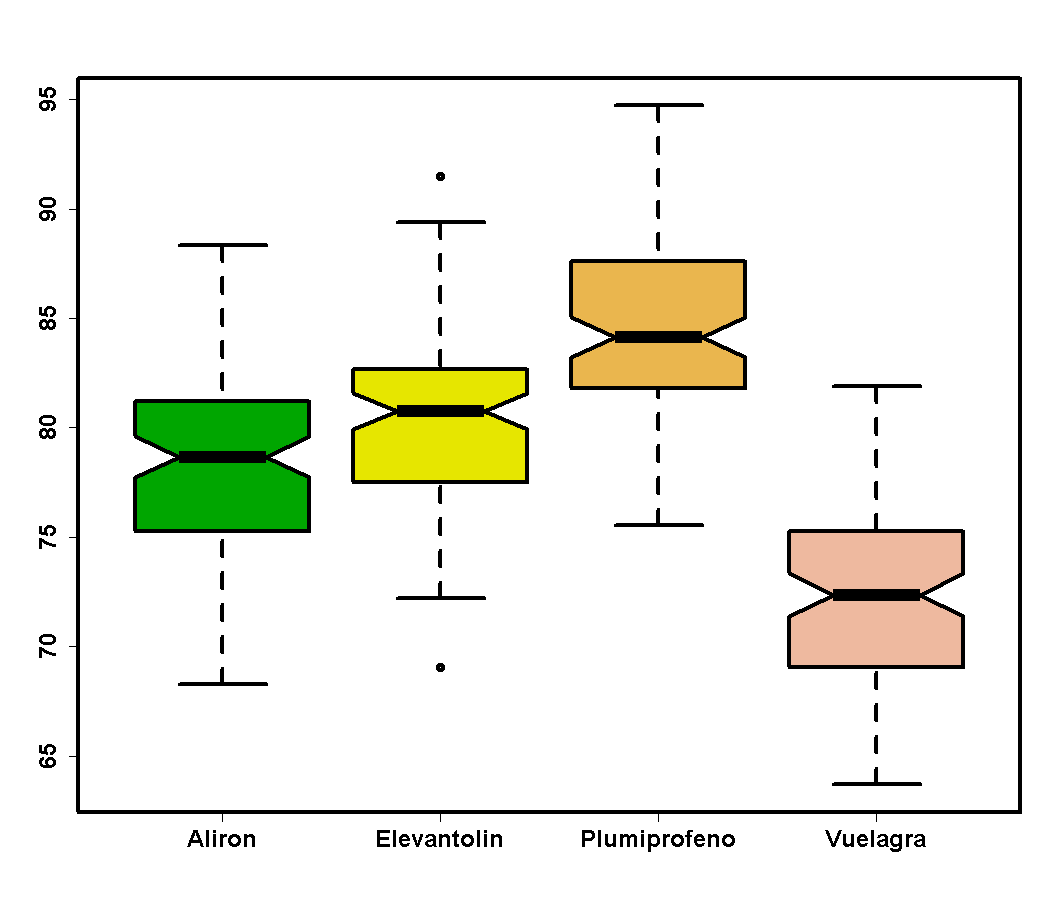
\includegraphics[width=9cm]{../fig/Tut11-01.png}
 \end{center}
\caption{Boxplots paralelos del Ejemplo \ref{curso-cap11:ejem:Anova01} del libro.}
\label{tut11:fig:BoxplotsParalelosEjemploAnova}
\end{figure}

Como puedes ver, estos diagramas de caja tienen una {\em muesca} o {\em bisel doble} alrededor de la mediana. La anchura de esa muesca viene a ser un análogo de los intervalos de confianza que conocemos, pero aplicado a la mediana en lugar de la media. El parámetro {\tt notch} controla la aparición de ese bisel doble o muesca en el diagrama de cajas. ¿Por qué lo hemos incluido en este caso? Pues porque, al tratarse de muestras grandes y, como veremos en la próxima sección, aproximadamente normales, la media y la mediana son muy similares. Y esos biseles permiten, de forma muy sencilla, evaluar gráficamente si existen diferencias significativas entre las medianas (y por consiguiente, en este ejemplo, entre las medias). La regla práctica que se aplica es que si los biseles correspondientes a dos niveles no se solapan entre sí (en vertical), entonces podemos sospechar que existen diferencias significativas entre las medianas correspondientes a esos dos niveles. Si quieres profundizar más en el uso y significado del parámetro {\tt notch} te recomendamos que consultes la ayuda de la función {\tt boxplot} de R.

Como puede verse, en este ejemplo tenemos razones para sospechar que existen diferencias significativas, dos a dos, en todos los casos: no hay dos niveles que tengan la misma media (aunque {\em Alirón} y {\em Elevantolín} tienen medias bastante similares). El gráfico también parece responder a la pregunta de cuál es el tratamiento más eficaz, ya que {\em Plumiprofeno} parece ser significativamente mejor que los demás. Volveremos sobre esa discusión en la Sección \ref{tut11:sec:ComparacionesDosaDos} (pág. \pageref{tut11:sec:ComparacionesDosaDos}).

\begin{ejercicio}
\label{tut11:ejercicio02}
Obten las figuras correspondientes para los ficheros de datos que hemos usado en el Ejercicio \ref{tut11:ejercicio01}, pág. \pageref{tut11:ejercicio01}.
%Soluciones en la página \pageref{tut11:ejercicio01:sol}.
\qed
\end{ejercicio}


\subsubsection*{Coeficiente de correlación lineal.}
\label{tut11:subsubsec:CoeficienteCorrelacionLineal}

Para completar el cálculo manual de la tabla Anova vamos a obtener el valor del coeficiente de correlación lineal y el valor del coeficiente de correlación ajustado que se describen en la Sección \ref{curso-cap11:subsec:CoeficienteCorrelacionAnova} del libro (pág. \pageref{curso-cap11:subsec:CoeficienteCorrelacionAnova}). El fichero {\tt Tut11-Anova-Basico.R} contiene asimismo instrucciones para calcular ``a mano'' esos coeficientes a partir de nuestros cálculos previos del modelo:
\begin{knitrout}
\definecolor{shadecolor}{rgb}{0.969, 0.969, 0.969}\color{fgcolor}\begin{kframe}
\begin{alltt}
\hlcom{#############################################}
\hlcom{# Coeficiente de correlacion.}
\hlcom{#############################################}

\hlcom{# El coeficiente de correlacion lineal es:}

\hlstd{(R2} \hlkwb{=} \hlstd{SSmodelo} \hlopt{/} \hlstd{SStotal)}
\end{alltt}
\begin{verbatim}
## [1] 0.53066
\end{verbatim}
\begin{alltt}
\hlcom{# Mientras que el coeficiente de correlacion lineal ajustado es:}

\hlstd{(adjR2} \hlkwb{=} \hlnum{1} \hlopt{-} \hlstd{((SSresidual} \hlopt{/} \hlstd{(N} \hlopt{-} \hlstd{k))} \hlopt{/} \hlstd{(SStotal} \hlopt{/} \hlstd{(N} \hlopt{-} \hlnum{1}\hlstd{))))}
\end{alltt}
\begin{verbatim}
## [1] 0.52711
\end{verbatim}
\end{kframe}
\end{knitrout}

\begin{ejercicio}
\label{tut11:ejercicio03}
Obten la tabla Anova y el coeficiente de correlación lineal para cada uno de los ficheros de datos que hemos usado en el Ejercicio \ref{tut11:ejercicio01}, pág. \pageref{tut11:ejercicio01}. %Soluciones en la página \pageref{tut11:ejercicio01:sol}.
\qed
\end{ejercicio}


\subsection{Tabla Anova con las funciones {\tt lm} y {\tt anova} de R. Coeficiente de correlación y coeficientes del modelo lineal.}
\label{tut11:subsec:TablaAnovaConFuncionAnovaR}

Aunque en la sección anterior hemos obtenido uno por uno los elementos que componen la Tabla de un contraste Anova unifactorial, esa no es, desde luego, la forma habitual de proceder. En la práctica resulta mucho más cómodo recurrir a las funciones que proporciona R y que en apenas dos líneas de código reproducen todos esos pasos que, laboriosamente, hemos ido dando.

Concretamente, el primer paso es utilizar la función {\tt lm}, que tuvimos ocasión de conocer en el Tutorial10, y después aplicaremos la función {\tt anova} al modelo resultante de {\tt lm}. Hacemos:

\begin{knitrout}
\definecolor{shadecolor}{rgb}{0.969, 0.969, 0.969}\color{fgcolor}\begin{kframe}
\begin{alltt}
\hlcom{##################################################}
\hlcom{# Ahora vamos a obtener los mismos resultados}
\hlcom{# usando las funciones lm,  anova y summary:}
\hlcom{##################################################}

\hlstd{datos.lm} \hlkwb{=} \hlkwd{lm}\hlstd{(Respuesta} \hlopt{~} \hlstd{Tratamiento,} \hlkwc{data} \hlstd{= datos)}

\hlkwd{anova}\hlstd{(datos.lm)}
\end{alltt}
\begin{verbatim}
## Analysis of Variance Table
## 
## Response: Respuesta
##              Df Sum Sq Mean Sq F value Pr(>F)    
## Tratamiento   3   7897    2632     149 <2e-16 ***
## Residuals   396   6984      18                   
## ---
## Signif. codes:  0 '***' 0.001 '**' 0.01 '*' 0.05 '.' 0.1 ' ' 1
\end{verbatim}
\end{kframe}
\end{knitrout}

Una ventaja añadida de nuestro trabajo de la sección anterior es que ahora resulta muy fácil interpretar esta Tabla Anova, y ver cuál es la información que R produce como respuesta.

\begin{itemize}
  \item Las dos primeras columnas contienen, respectivamente, los grados de libertad {\tt Df}, y las sumas de cuadrados del modelo y residual, en la que se denomina {\tt Sum Sq}.
  \item La única columna de la tabla que puede despistarnos un poco es la tercera, que tiene como encabezamiento {\tt Mean Sq}, pero en ella aparecen, simplemente, el numerador y el denominador, respectivamente, del Estadístico $\Xi$, que a su vez aparece en la columna denominada {\tt F value}.
  \item El p-valor aparece en la columna {\tt Pr(>F)} (el símbolo, como ves, indica la cola derecha de la distribución $F$). R utiliza, como en otros casos, un código de asteriscos para indicar el tamaño del p-valor que se ha obtenido. En este caso, el valor {\tt 2.2e-16} que aparece no es, realmente, el p-valor, sino una forma de indicarnos que se ha alcanzado un valor más pequeño que el límite de precisión de R para distinguirlo del cero (y que, desde luego, justifica sobradamente los tres asteriscos).
\end{itemize}

Otra forma de obtener información útil adicional sobre el modelo es usando la función {\tt summary}.
\begin{knitrout}
\definecolor{shadecolor}{rgb}{0.969, 0.969, 0.969}\color{fgcolor}\begin{kframe}
\begin{alltt}
\hlkwd{summary}\hlstd{(datos.lm)}
\end{alltt}
\begin{verbatim}
## 
## Call:
## lm(formula = Respuesta ~ Tratamiento, data = datos)
## 
## Residuals:
##    Min     1Q Median     3Q    Max 
## -11.37  -2.81   0.11   2.77  11.11 
## 
## Coefficients:
##                         Estimate Std. Error t value Pr(>|t|)    
## (Intercept)               78.399      0.420  186.68  < 2e-16 ***
## TratamientoElevantolin     2.000      0.594    3.37  0.00083 ***
## TratamientoPlumiprofeno    6.001      0.594   10.10  < 2e-16 ***
## TratamientoVuelagra       -6.299      0.594  -10.61  < 2e-16 ***
## ---
## Signif. codes:  0 '***' 0.001 '**' 0.01 '*' 0.05 '.' 0.1 ' ' 1
## 
## Residual standard error: 4.2 on 396 degrees of freedom
## Multiple R-squared:  0.531,	Adjusted R-squared:  0.527 
## F-statistic:  149 on 3 and 396 DF,  p-value: <2e-16
\end{verbatim}
\end{kframe}
\end{knitrout}



Volviendo a los resultados de la función {\tt summary}, cabe preguntarse qué representan los números que aparecen en el apartado {\tt Coefficients}. Pero para hacerlo tendremos que esperar un poco, porque necesitamos las ideas sobre {\em constrastes} que se discuten en la Sección \ref{curso-cap11:subsubsec:IntroduccionContrastes} del libro (pág. \pageref{curso-cap11:subsubsec:IntroduccionContrastes}) y en la Sección \ref{tut11:sec:IntroduccionALosContrastes} de este tutorial (pág. \pageref{tut11:sec:IntroduccionALosContrastes}). En cualquier caso, para adelantar un poco esas ideas, puedes observar que el primer valor que aparece en la fila {\tt Intercept} es la media $\bar X_{{\mbox{\bf\large$\cdot$}}1}=78.40$ del primer nivel (por orden alfabético), el {\em Aliron}. Los valores iniciales de las siguientes tres filas son {\em las diferencias} entre este valor y las medias de los restantes tres niveles:
\[
\begin{cases}
\bar X_{{\mbox{\bf\large$\cdot$}}2} - \bar X_{{\mbox{\bf\large$\cdot$}}1} =  80.40 - 78.40 = 2.00\\
\bar X_{{\mbox{\bf\large$\cdot$}}3} - \bar X_{{\mbox{\bf\large$\cdot$}}1} =  84.40 - 78.40 = 6.00\\
\bar X_{{\mbox{\bf\large$\cdot$}}4} - \bar X_{{\mbox{\bf\large$\cdot$}}1} =  72.10 - 78.40 = -6.30\\
\end{cases}
\]
Más adelante, en la Sección \ref{tut11:sec:IntroduccionALosContrastes} de este Tutorial, veremos por qué nos pueden interesar estos valores, y qué significan las restantes columnas de la tabla en la que aparecen. En particular, aprenderemos a controlar el proceso. Al construir esta tabla R ha tomado muchas decisiones de manera automática. Por ejemplo, ha decidido comparar $\bar X_{{\mbox{\bf\large$\cdot$}}1}$ con los demás. Esas decisiones pueden no coincidir con nuestros deseos a la hora de analizar un diseño experimental concreto. A lo mejor a nosotros nos interesa más comparar $\bar X_{{\mbox{\bf\large$\cdot$}}2}$ frente a los restantes valores, o queremos averiguar  si las medias están ordenadas de determinada manera, etc.


\section{Verificando las condiciones del Anova unifactorial en R}
\label{tut11:sec:VerificandoCondicionesAnovaR}

Puesto que la discusión de las condiciones de aplicabilidad del contraste Anova que hemos hecho en la Sección  \ref{curso-cap11:subsec:AnalisisCondicionesAnova} (pág. \pageref{curso-cap11:subsec:AnalisisCondicionesAnova}) del libro ha sido bastante superficial, no vamos a entrar aquí en un análisis muy minucioso de cómo usar R para chequear esas condiciones. Nos vamos a limitar a las ideas más básicas. Para facilitar el trabajo, vamos a incluir el código necesario en un fichero, llamado
\begin{center}
\fichero{./code/Tut11-Anova-Avanzado.R}{Tut11-Anova-Avanzado.R}
\end{center}
Este fichero contiene parte del mismo código que hemos visto en el fichero {\tt Tut11-Anova-Basico.R}, del que hemos eliminado la parte de cálculo paso a paso de la Tabla Anova, dejando sólo la versión que usa las funciones {\tt lm} y {\tt anova}. Y hemos añadido código para un análisis más detallado del contraste Anova, que vamos a describir en ésta y en la próxima sección.




\subsubsection*{Histogramas por niveles (grupos).}

Hemos visto ya como obtener diagramas de cajas paralelos de la respuesta para los distintos grupos (niveles) del factor {\tt Tratamiento}. Esos diagramas de cajas, si los grupos son suficientemente numerosos, pueden servir para verificar gráficamente la condición de normalidad. Además, la dispersión dentro de cada uno de los grupos no debería ser llamativamente distinta, para que se cumpla la condición de homogeneidad de varianzas. Se puede hacer un estudio similar a partir de los histogramas de la respuesta en cada uno de los grupos. Para obtener todos los histogramas, de nuevo vamos a solicitar la ayuda de {\tt tapply}. El código, del que enseguida comentaremos algunos detalles, es este:
\begin{knitrout}
\definecolor{shadecolor}{rgb}{0.969, 0.969, 0.969}\color{fgcolor}\begin{kframe}
\begin{alltt}
\hlcom{# Histogramas de cada uno de los grupos}
\hlkwd{par}\hlstd{(}\hlkwc{mfrow}\hlstd{=}\hlkwd{c}\hlstd{(k}\hlopt\hlnum{2}\hlopt{+}\hlstd{k}\hlopt\hlnum{2}\hlstd{,}\hlnum{2}\hlstd{),}\hlkwc{font.axis}\hlstd{=}\hlnum{1.5}\hlstd{,}\hlkwc{cex.axis}\hlstd{=}\hlnum{1.5}\hlstd{,}\hlkwc{lwd}\hlstd{=}\hlnum{2}\hlstd{,}\hlkwc{font.lab}\hlstd{=}\hlnum{2}\hlstd{,}\hlkwc{cex.lab}\hlstd{=}\hlnum{1.5}\hlstd{)}
\hlstd{histogramas} \hlkwb{=} \hlkwd{tapply}\hlstd{(datos}\hlopt{$}\hlstd{Respuesta,datos}\hlopt{$}\hlstd{Tratamiento, hist,} \hlkwc{breaks}\hlstd{=}\hlnum{10}\hlstd{,}
       \hlkwc{main}\hlstd{=}\hlstr{""}\hlstd{,} \hlkwc{ylab}\hlstd{=}\hlstr{"Frecuencia"}\hlstd{,} \hlkwc{xlab}\hlstd{=}\hlstr{""}\hlstd{,} \hlkwc{col}\hlstd{=}\hlkwd{heat.colors}\hlstd{(}\hlnum{10}\hlstd{))}
\hlkwd{par}\hlstd{(}\hlkwc{mfrow}\hlstd{=}\hlkwd{c}\hlstd{(}\hlnum{1}\hlstd{,}\hlnum{1}\hlstd{))}
\end{alltt}
\end{kframe}
\end{knitrout}

y el resultado puede verse en la Figura \ref{tut11:fig:HistogramasParalelosEjemploAnova}.
\begin{figure}[htb]
\begin{center}
    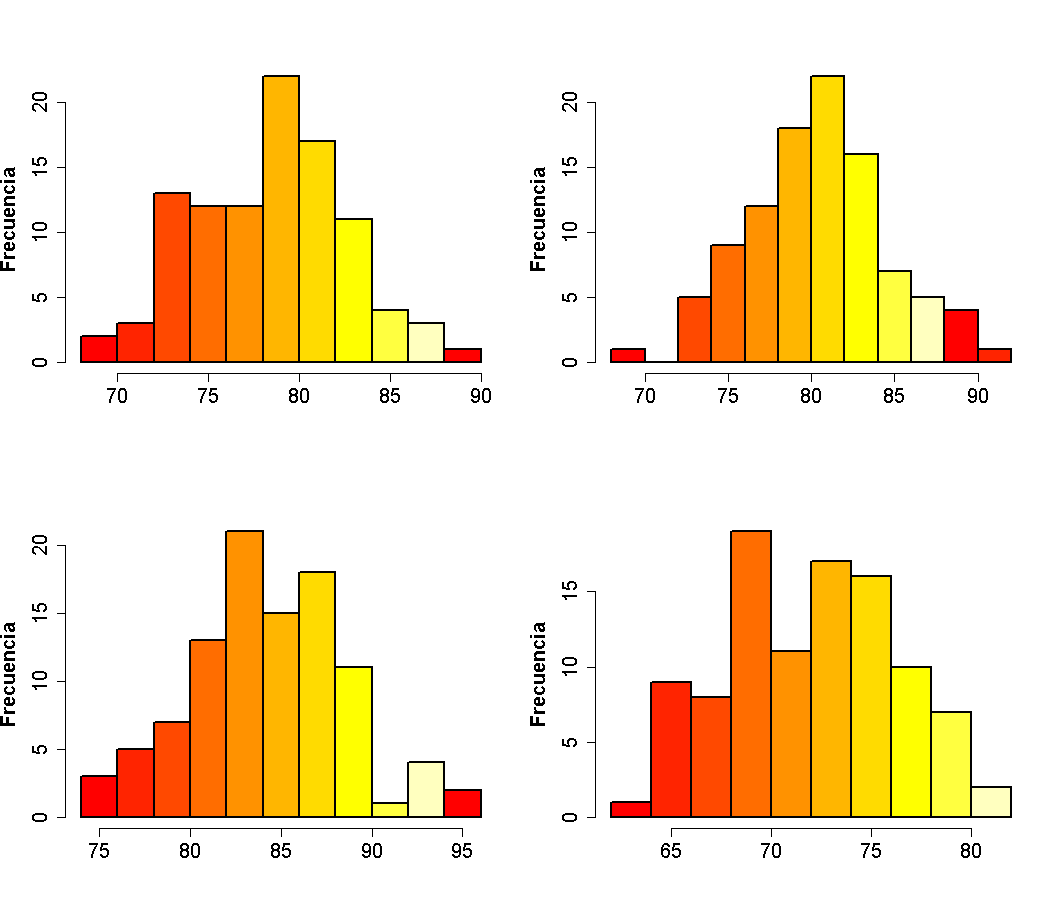
\includegraphics[width=14cm]{../fig/Tut11-02.png}
\end{center}
\caption{Histogramas paralelos del Ejemplo \ref{curso-cap11:ejem:Anova01} del libro.}
\label{tut11:fig:HistogramasParalelosEjemploAnova}
\end{figure}

Algunos comentarios sobre esa figura y sobre el código que hemos usado para generarla:
\begin{itemize}
  \item Los cuatro histogramas que hemos obtenido, uno por nivel, no parecen indicar que haya ningún problema evidente con las condiciones de normalidad y homogeneidad de las varianzas. Dicho de otra manera, no hay ninguno que sea escandalosamente no normal. Y muchas veces nos tendremos que conformar con eso y con otra información adicional que nos permita suponer que las poblaciones son normales. Por ejemplo, ya hemos comentado que muchos fenómenos naturales se ajustan a la distribución normal y podemos usar la intuición de que el fenómeno que estudiamos es uno de ellos. En términos generales, los cuatro histogramas tienen forma de campana, con aproximadamente el mismo perfil.
  \item Las dos líneas con {\tt par} que rodean a la línea con {\tt tapply} sirven para fijar parámetros del gráfico. En concreto, la primera usa el parámetro, de aspecto algo cabalístico,
      \begin{center}
      \verb#mfrow=c(k%/%2+k%%2,2)#
      \end{center}
      para crear una {\em matriz de gráficos}. En el ejemplo concreto que estamos usando, los gráficos son cuatro, y podríamos colocarlos en una matriz $2\times 2$ con \verb#mfrow=c(2,2)#. Pero, puesto que queremos un código que funcione en el caso general, tendremos {\tt k} niveles, y para colocarlos en una matriz de dos columnas tenemos que averiguar el número de filas. Eso es lo que hacen esas instrucciones misteriosas. Concretamente, \verb#k%/%2# es el cociente de la división de $k$ entre $2$, mientras que  \verb#k%/%2#       es el resto. De esa forma, si tenemos, por ejemplo, $k=9$ niveles, al ser $k=2\cdot 4+1$, sabremos que necesitamos $cociente+resto=4+1=5$ filas para los nueve gráficos (con dos columnas, recuerda). El resto de los valores que aparecen en el primer {\tt par} son simplemente ``decorativos'': tamaños de letra, tipografía, etiquetado, etc. El {\tt mfrow=c(1,1)} que aparece en el segundo par sirve para devolver los gráficos de R a su estado anterior (una matriz $1\times 1$ de gráficos).

  \item En la llamada a {\tt tapply} la parte esencial es
      \begin{center}
      \verb#tapply(datos$Respuesta,datos$Tratamiento,hist,breaks=10,#
      \end{center}
      El resto es casi todo, de nuevo, ``decorativo''. Hemos pasado a {\tt hist} la opción {\tt breaks=10} para que todos los histogramas tuvieran el mismo número de columnas, lo que ayuda a comprobar si sus perfiles son similares.

\end{itemize}

\subsubsection*{Análisis de los residuos.}

Como sabemos por nuestra experiencia en el modelo de regresión lineal el análisis de las condiciones de aplicabilidad del contraste Anova pasa por un análisis de los residuos. En esta incursión tan breve que estamos haciendo, nos vamos a limitar al análisis gráfico de los residuos, usando las herramientas que R nos proporciona. En particular, vamos a usar una nueva función, la función  {\tt aov} (de {\em analysis of variance}), que entre otras cosas nos va a permitir obtener ese análisis gráfico de los residuos. Para que R calcule los residuos y prepare esos gráficos, empezamos haciendo:

\begin{knitrout}
\definecolor{shadecolor}{rgb}{0.969, 0.969, 0.969}\color{fgcolor}\begin{kframe}
\begin{alltt}
\hlcom{#########################################}
\hlcom{# Gr<U+00E1>ficos para el an<U+00E1>lisis mediante}
\hlcom{# residuos de las hip<U+00F3>tesis del modelo.}
\hlcom{#########################################}

\hlstd{datos.aov} \hlkwb{=} \hlkwd{aov}\hlstd{(datos}\hlopt{$}\hlstd{Respuesta} \hlopt{~} \hlstd{datos}\hlopt{$}\hlstd{Tratamiento, datos)}
\hlkwd{par}\hlstd{(}\hlkwc{mfrow}\hlstd{=}\hlkwd{c}\hlstd{(}\hlnum{2}\hlstd{,}\hlnum{2}\hlstd{),} \hlkwc{cex.axis}\hlstd{=}\hlnum{1.5}\hlstd{,} \hlkwc{lwd}\hlstd{=}\hlnum{2}\hlstd{,} \hlkwc{font.lab}\hlstd{=}\hlnum{1.5}\hlstd{)}
\hlkwd{plot}\hlstd{(datos.aov)}
\hlkwd{par}\hlstd{(}\hlkwc{mfrow}\hlstd{=}\hlkwd{c}\hlstd{(}\hlnum{1}\hlstd{,}\hlnum{1}\hlstd{))}
\end{alltt}
\end{kframe}
\end{knitrout}

El resultado se muestra en la Figura \ref{tut11:fig:AnalisisResiduosEjemploAnova}.
Ya sabemos cuál es la misión de las dos llamadas a {\tt par} que rodean a la función {\tt plot}. Con independencia del número de niveles R siempre produce cuatro gráficos para el análisis de los residuos, así que hemos decidido colocarlos en una matriz de gráficos $2\times 2$, usando {\tt mfrow} dentro de {\tt par}.

\begin{figure}[htb]
\begin{center}
    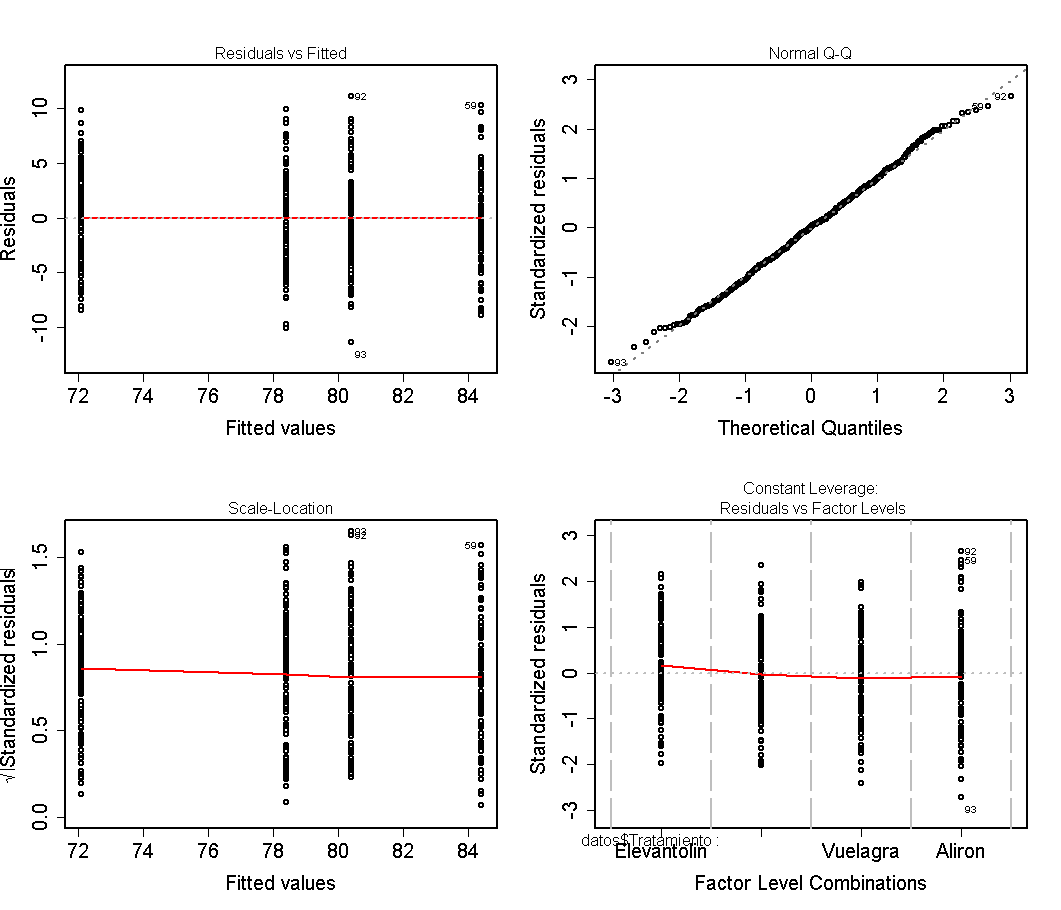
\includegraphics[width=15cm]{../fig/Tut11-03.png}
\end{center}
\caption{Análisis gráfico de los residuos para el Ejemplo \ref{curso-cap11:ejem:Anova01} del libro.}
\label{tut11:fig:AnalisisResiduosEjemploAnova}
\end{figure}


De esos cuatro gráficos, vamos a centrar nuestra atención en los dos de la primera fila.
\begin{itemize}
   \item El de la izquierda muestra los residuos frente a los valores que predice el modelo. Esos valores predichos, en el Anova unifactorial, no  son más que las medias de cada uno de los niveles; cuatro, para este ejemplo concreto. Por esa razón vemos cuatro grupos de puntos, con cada grupo situado, sobre el valor en el eje horizontal de cada una de las medias. Lo que debemos buscar, en este primer gráfico, para evaluar las condiciones de aplicabilidad de Anova, es si existe algún patrón apreciable en las distribuciones de los residuos, de forma que, por ejemplo, la dispersión de los residuos pudiera aumentar de izquierda a derecha (o viceversa). Es decir, buscamos la existencia de posibles patrones en forma de cuña, en el mismo sentido que vimos en la discusión en torno a la Figura \ref{curso-cap10:fig:AnalisisMedianteResiduosHomogeneidadVarianza} (pág. \pageref{curso-cap10:fig:AnalisisMedianteResiduosHomogeneidadVarianza}) del libro, para el caso del modelo de regresión lineal. Hay que tener en cuenta, por supuesto, que allí la variable explicativa era continua, mientras que aquí es discreta, y que eso se traduce en que los residuos se agrupan en las trazas verticales que hemos comentado, una por nivel.

  \item El segundo gráfico de la primera fila es un {\tt qqplot} de los residuos, que se usa para obtener una nueva verificación de la hipótesis de normalidad de los residuos. En este caso, los residuos se ajustan muy satisfactoriamente a la recta, así que no parece que debamos preocuparnos por esa condición.

\end{itemize}


Naturalmente, hay mucho más que decir sobre este tema. Más allá de un análisis gráfico, existen
contrastes formales que pueden utilizarse para verificar las condiciones de Anova. Y no hemos
hecho, por ejemplo, una discusión sobre la posible existencia de valores atípicos o influyentes,
similar a la que hicimos en el caso de la regresión lineal. En el Apéndice \ref{curso-apendice:MasAlla} del libro (pág. \pageref{curso-apendice:MasAlla}) se pueden
encontrar referencias a tratamientos más avanzados de Anova.

\begin{ejercicio}
\label{tut11:ejercicio04}
Aplica el fichero {\tt Tut11-Anova-Avanzado.R} para construir y analizar los modelos Anova que hemos construido en el Ejercicio \ref{tut11:ejercicio01}, pág. \pageref{tut11:ejercicio01}. ¿Qué conclusiones obtienes sobre la validez de estos modelos?
 %Soluciones en la página \pageref{tut11:ejercicio04:sol}.
\qed
\end{ejercicio}


\section{Comparaciones dos a dos a posteriori}
\label{tut11:sec:ComparacionesDosaDos}

 Una vez que sabemos que el contraste Anova ha sido significativo, y que, por tanto, las medias de los diferentes niveles no son todas iguales, la pregunta natural es: ¿qué parejas son significativamente diferentes?

Hay, de nuevo, mucho más que decir sobre este tema de lo que vamos a presentar aquí. Por ejemplo,
una situación frecuente es aquella en la que existe un grupo (denominado {\sf grupo de control} o,
simplemente, {\sf control}) y queremos comparar la media de los demás grupos con la de ese grupo de
control. Este tema está íntimamente relacionado con el diseño del experimento subyacente a este
modelo Anova, y para tratarlo con más detalle deberíamos entrar en esa discusión y en la noción de
{\sf matriz de contraste}, de la que hablaremos en la Sección \ref{tut11:sec:IntroduccionALosContrastes}. Aquí nos vamos a limitar a presentar las ideas más básicas sin entrar a fondo en la discusión del diseño del experimento. Como hemos dicho anteriormente, el Apéndice \ref{curso-apendice:MasAlla} del libro (pág. \pageref{curso-apendice:MasAlla}) contiene referencias a tratamientos completos del Diseño Experimental.

En R, la herramienta más sencilla para obtener ese tipo de comparaciones dos a dos es la función {\tt pairwise.t.test}.  Al usarla, debemos tener en cuenta que es necesario reajustar los p-valores, como hemos comentado en la Sección \ref{curso-cap11:sec:AnovaSignificativoComparacionesDosaDos}, para evitar la posibilidad de cometer un error de Tipo I (un falso positivo, rechazando la hipótesis nula, que nos llevaría a asegurar que hay diferencias entre los niveles del tratamiento), debido simplemente a la repetición de un número alto de contrastes. Hay muchos métodos para realizar ese ajuste, cada uno con sus ventajas e inconvenientes. Aquí vamos a adoptar un enfoque muy clásico, y vamos a utilizar el método de Bonferroni, que hemos descrito en la Sección \ref{curso-cap11:subsec:Bonferroni} del libro (pág. \pageref{curso-cap11:subsec:Bonferroni}) y que multiplica cada p-valor por el número de comparaciones que se han realizado.
Para hacer esto en R, con los datos del Ejemplo \ref{curso-cap11:ejem:Anova01} de los frailecillos, usamos el siguiente código:
\begin{knitrout}
\definecolor{shadecolor}{rgb}{0.969, 0.969, 0.969}\color{fgcolor}\begin{kframe}
\begin{alltt}
\hlcom{#########################################}
\hlcom{# Comparaciones a posteriori, dos a dos}
\hlcom{#########################################}
\hlcom{# En caso de un Anova significativo, podemos comparar los grupos dos a dos}
\hlcom{# Los p-valores de las comparaciones se obtienen con este comando:}

\hlstd{(ptt}\hlkwb{=}\hlkwd{pairwise.t.test}\hlstd{(datos}\hlopt{$}\hlstd{Respuesta, datos}\hlopt{$}\hlstd{Tratamiento,}
                     \hlkwc{p.adj}\hlstd{=}\hlstr{"bonferroni"}\hlstd{,} \hlkwc{pool.sd}\hlstd{=}\hlnum{FALSE}\hlstd{))}
\end{alltt}
\begin{verbatim}
## 
## 	Pairwise comparisons using t tests with non-pooled SD 
## 
## data:  datos$Respuesta and datos$Tratamiento 
## 
##              Aliron Elevantolin Plumiprofeno
## Elevantolin  0.005  -           -           
## Plumiprofeno <2e-16 1e-09       -           
## Vuelagra     <2e-16 <2e-16      <2e-16      
## 
## P value adjustment method: bonferroni
\end{verbatim}
\end{kframe}
\end{knitrout}
Fíjate que la respuesta contiene seis p-valores, porque al trabajar con cuatro niveles tenemos
\[\binom{4}{2} = 6\]
posibles parejas para comparar. Por ejemplo, el p-valor (ajustado mediante el método de Bonferroni) de la comparación entre {\em Plumiprofeno} y {\em Elevantolín} aparece como {\tt 1e-09}. Como decíamos, podemos conseguir una información más detallada así:
\begin{knitrout}
\definecolor{shadecolor}{rgb}{0.969, 0.969, 0.969}\color{fgcolor}\begin{kframe}
\begin{alltt}
\hlstd{ptt}\hlopt{$}\hlstd{p.value}
\end{alltt}
\begin{verbatim}
##                  Aliron Elevantolin Plumiprofeno
## Elevantolin  5.4566e-03          NA           NA
## Plumiprofeno 7.6636e-19  1.0408e-09           NA
## Vuelagra     2.5313e-20  1.4943e-30    1.148e-50
\end{verbatim}
\end{kframe}
\end{knitrout}
Y así vemos los p-valores con más precisión. Realmente, muchas veces no es necesario hacer esto, porque a menudo sólo nos interesa la magnitud del p-valor, y no necesitamos conocerlo con precisión. No obstante, esta vez lo hemos hecho así para que resulte más fácil ver la corrección de Bonferroni en acción. Hagamos una de esas seis comparaciones individuales por separado, usando el estadístico $\Upsilon$ que aparece en la Ecuación \ref{curso-cap11:ecu:EstadisticoComparacionesPostHoc} del libro (pág. \pageref{curso-cap11:ecu:EstadisticoComparacionesPostHoc}):
$$\Upsilon =
\dfrac{\bar X_{{\mbox{\bf\large$\cdot$}}i}-\bar X_{{\mbox{\bf\large$\cdot$}}j}}{
{\sqrt{s_{\mbox{pond}}^2\cdot\left(\dfrac{1}{n_i}+\dfrac{1}{n_j}\right)}}},$$
donde $s_{\mbox{pond}}^2$ es la {\em cuasidesviación ponderada} (en inglés, {\em pooled sd}), que aparece en la Ecuación \ref{curso-cap11:ecu:CuasivarianzaPonderadaComparacionesPostHoc} del libro (pág. \pageref{curso-cap11:ecu:CuasivarianzaPonderadaComparacionesPostHoc}) y que se definide mediante
$$
s_{\mbox{pond}}^2=\dfrac{SS_{\mbox{\tiny residual}}}{N-k}
$$
Concretamente, vamos a usar esto para calcular el p-valor para el contraste de igualdad de medias entre {\em Plumiprofeno} y {\em Elevantolín}. Recuerda que el número de observaciones en cada nivel del factor está almacenado en el vector {\tt replicas} de R. El cálculo es este:
\begin{knitrout}
\definecolor{shadecolor}{rgb}{0.969, 0.969, 0.969}\color{fgcolor}\begin{kframe}
\begin{alltt}
\hlstd{(NumEstadistico} \hlkwb{=} \hlstd{mediasPorNivel[}\hlnum{2}\hlstd{]} \hlopt{-} \hlstd{mediasPorNivel[}\hlnum{3}\hlstd{]  )}
\end{alltt}
\begin{verbatim}
## Elevantolin 
##     -4.0004
\end{verbatim}
\begin{alltt}
\hlstd{(pooledSd} \hlkwb{=} \hlkwd{sqrt}\hlstd{(SSresidual}\hlopt{/}\hlstd{(N}\hlopt{-}\hlstd{k)))}
\end{alltt}
\begin{verbatim}
## [1] 4.1997
\end{verbatim}
\begin{alltt}
\hlstd{(denomEstadistico} \hlkwb{=} \hlkwd{sqrt}\hlstd{(pooledSd}\hlopt{^}\hlnum{2} \hlopt{*} \hlstd{((}\hlnum{1} \hlopt{/} \hlstd{replicas[}\hlnum{2}\hlstd{])} \hlopt{+} \hlstd{(}\hlnum{1} \hlopt{/} \hlstd{replicas[}\hlnum{3}\hlstd{]))))}
\end{alltt}
\begin{verbatim}
## Elevantolin 
##     0.59393
\end{verbatim}
\begin{alltt}
\hlstd{(Estadistico} \hlkwb{=} \hlstd{NumEstadistico} \hlopt{/} \hlstd{denomEstadistico)}
\end{alltt}
\begin{verbatim}
## Elevantolin 
##     -6.7355
\end{verbatim}
\end{kframe}
\end{knitrout}
No te preocupes por el nombre que aparece sobre el valor del estadístico, R lo arrastra porque {\tt replicas} es una tabla con nombres. Ahora podemos usar la Ecuación \ref{curso-cap11:ecu:pValorAjusteBonferroni} del libro (pág. \pageref{curso-cap11:ecu:pValorAjusteBonferroni}) para calcular el p-valor con el ajuste de Bonferroni:

\begin{knitrout}
\definecolor{shadecolor}{rgb}{0.969, 0.969, 0.969}\color{fgcolor}\begin{kframe}
\begin{alltt}
\hlstd{(NumComp} \hlkwb{=} \hlkwd{choose}\hlstd{(k,} \hlnum{2}\hlstd{))}
\end{alltt}
\begin{verbatim}
## [1] 6
\end{verbatim}
\begin{alltt}
\hlstd{(pV} \hlkwb{=} \hlkwd{min}\hlstd{(NumComp} \hlopt{*} \hlnum{2} \hlopt{*} \hlstd{(}\hlnum{1} \hlopt{-} \hlkwd{pt}\hlstd{(}\hlkwd{abs}\hlstd{(Estadistico),} \hlkwc{df} \hlstd{= N} \hlopt{-} \hlstd{k)),} \hlnum{1}\hlstd{))}
\end{alltt}
\begin{verbatim}
## [1] 3.4608e-10
\end{verbatim}
\end{kframe}
\end{knitrout}
Y comparamos con el resultado que obtuvimos en {\tt pairwise.t.test} para esa pareja de niveles, para comprobar que coincide con nuestro cálculo ``manual'':
\begin{knitrout}
\definecolor{shadecolor}{rgb}{0.969, 0.969, 0.969}\color{fgcolor}\begin{kframe}
\begin{alltt}
\hlstd{ptt}\hlopt{$}\hlstd{p.value[}\hlnum{2}\hlstd{,} \hlnum{2}\hlstd{]}
\end{alltt}
\begin{verbatim}
## [1] 1.0408e-09
\end{verbatim}
\end{kframe}
\end{knitrout}
El método de Bonferroni es, como hemos dicho, sólo una de las posibilidades. Su mayor limitación estriba en el hecho de que es un método de los denominados ``conservadores''. Es decir, que sacrifica excesivamente la potencia (en el sentido del Capítulo \ref{curso-cap07:sec:PotenciaContraste}), con el fin de evitar los falsos positivos. Pero tiene la virtud, como hemos puesto de manifiesto, de ser conceptualmente muy sencillo y fácil de aplicar.

A la luz de estos resultados puede ser una buena idea regresar a la Figura \ref{tut11:fig:BoxplotsParalelosEjemploAnova} (pág. \pageref{tut11:fig:BoxplotsParalelosEjemploAnova}), en la que hemos mostrado los diagramas de caja biselados de este mismo ejemplo, y tratar de ver si los p-valores que hemos obtenido coinciden con las conclusiones que hubiéramos podido extraer de ese análisis gráfico.

\begin{ejercicio}
\label{tut11:ejercicio05}
Usa código como el que hemos visto en esta sección para comprobar los resultados que aparecen en los Ejemplos \ref{curso-cap11:ejem:BonferroniMediasNoTodasDistintas} (pág. \pageref{curso-cap11:ejem:BonferroniMediasNoTodasDistintas}) y \ref{curso-cap11:ejem:AnovaSignificativoPostHocNoSignificativo} (pág. \pageref{curso-cap11:ejem:AnovaSignificativoPostHocNoSignificativo}) del libro.
% Soluciones en la página \pageref{tut11:ejercicio05:sol}.
\qed
\end{ejercicio}

\subsubsection*{Representaciones gráficas para las comparaciones entre grupos.}

Vamos a ver ahora el código necesario para obtener una representación gráfica como la de la Figura \ref{curso-cap11:fig:BonferroniMediasNoTodasDistintasBoxplotsGrupos} del libro (pág. \pageref{curso-cap11:fig:BonferroniMediasNoTodasDistintasBoxplotsGrupos}), que permite identificar fácilmente cuáles de las difernecias entre las medias de los niveles han resultado significativamente diferentes. Además, el código que incluimos permite obtener una representación alternativa de esa situación, como la de la Figura \ref{tut11:fig:DiagramaAlternativoEjemploPostHocAnova}

\begin{figure}[htb]
\begin{center}
    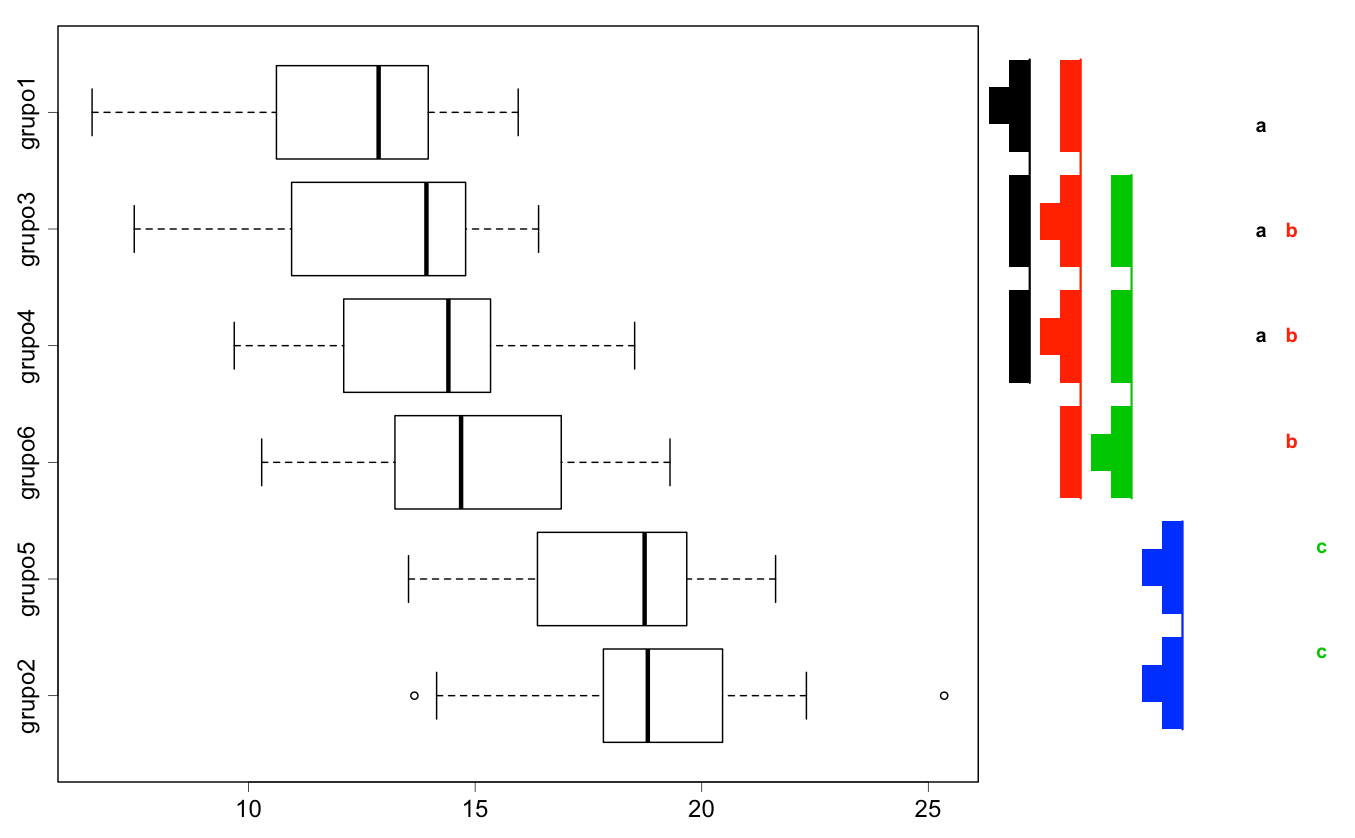
\includegraphics[width=12cm]{../fig/Tut11-06.png}
\end{center}
\caption{Otra representación de las comparaciones dos a dos para el Ejemplo \ref{curso-cap11:ejem:BonferroniMediasNoTodasDistintas} del libro.}
\label{tut11:fig:DiagramaAlternativoEjemploPostHocAnova}
\end{figure}


No vamos a entrar en detalles sobre este código, porque eso nos ocuparía demasiado espacio. Remitimos al lector interesado a la documentación de la librería {\tt multcomp}. El código aparece en el fichero {\tt Tut11-Anova-Avanzado.R} del que ya hemos hablado, dentro de un bloque titulado {\em Comparaciones a posteriori, representaciones gráficas}. Para utilizar esa parte del fichero hay que hacer lo siguiente:

\begin{itemize}
  \item Para empezar, por supuesto, fijar el directorio de trabajo y el nombre del fichero de datos.
  \item Asegurarnos de que hemos instalado las librerías {\tt multcomp} y {\tt multcompView} de R.
  \item Descomentar las líneas de código del bloque de comandos {\em Comparaciones a posteriori, representaciones gráficas}.
\end{itemize}

\begin{ejercicio}
\label{tut11:ejercicio06}
Haz esto con los datos de los Ejemplos \ref{curso-cap11:ejem:BonferroniMediasNoTodasDistintas} (pág. \pageref{curso-cap11:ejem:BonferroniMediasNoTodasDistintas}) y \ref{curso-cap11:ejem:AnovaSignificativoPostHocNoSignificativo} (pág. \pageref{curso-cap11:ejem:AnovaSignificativoPostHocNoSignificativo}) del libro.
% Soluciones en la página \pageref{tut11:ejercicio06:sol}.
\qed
\end{ejercicio}

\subsubsection*{Comentarios sobre los denominados {\sf bargraphs}}

Los contrastes de diferencias de medias como el Anova se acompañan a menudo, en las publicaciones científicas, de diagramas de columnas con barras de error ({\em bargraphs with error bars}, en inglés), como el que aquí hemos incluido en la Figura \ref{tut11:fig:BargraphEjemploAnova}. Estos diagramas se obtienen con mucha (demasiada) facilidad en las hojas de cálculo, lo cual sin duda explica parte de su popularidad. En el libro, concretamente en la página \pageref{curso-cap09:fig:GraficoBarrasError} hemos desaconsejado con insistencia el uso de este tipo de gráficos. Y ahora queremos volver a argumentar los problemas que merman la efectividad de estas gráficas para transmitir información veraz relativa a las diferencias entre las medias de los distintos tratamientos.

Las denominadas {\sf barras de error} son esas figuras con forma de I que aparecen en la parte superior de cada columna. Uno de los problemas con este tipo de gráficas es que las barras de error ni siquiera representan intervalos de confianza para la media de cada uno de los grupos, por lo que no es correcto usarlas para concluir diferencias significativas entre las medias de esos grupos. Además, no tiene mucho sentido usar una columna para indicar el valor de una media. Como vimos en en el primer capítulo del curso, los diagramas de columnas son adecuados para representar {\em frecuencias}, y su uso aquí resulta confuso. A menudo el nivel base de las columnas no tiene ningún significado especial, y fijarlo arbitrariamente en $0$ puede ser simplemente eso, una arbitrariedad, que además puede tener un impacto negativo en la capacidad del gráfico para transmitir la información relevante. Recomendamos, como alternativa, gráficos basados en intervalos de confianza, como el que aparece en la Figura 171, pág. 135 del libro {\em Introductory Statistics with R}, de Peter Dalgaard (ver la referencia en la Bibliografía del libro), y que son similares al que aquí incluimos en la Figura \ref{tut11:fig:DiagramaAlternativoEjemploAnova}. En cualquier caso, El fichero {\tt Tut11-Anova-Avanzado.R} contiene código para generar ambos tipos de gráficos.

%Puedes encontrar una discusión más amplia de este asunto en el artículo:
%
%{\em Lane, D. M., \& Sándor, A.} (2009). Designing better graphs by including distributional information and integrating words, numbers, and images. Psychological methods, 14(3), 239.

\begin{figure}[htb]
\begin{center}
    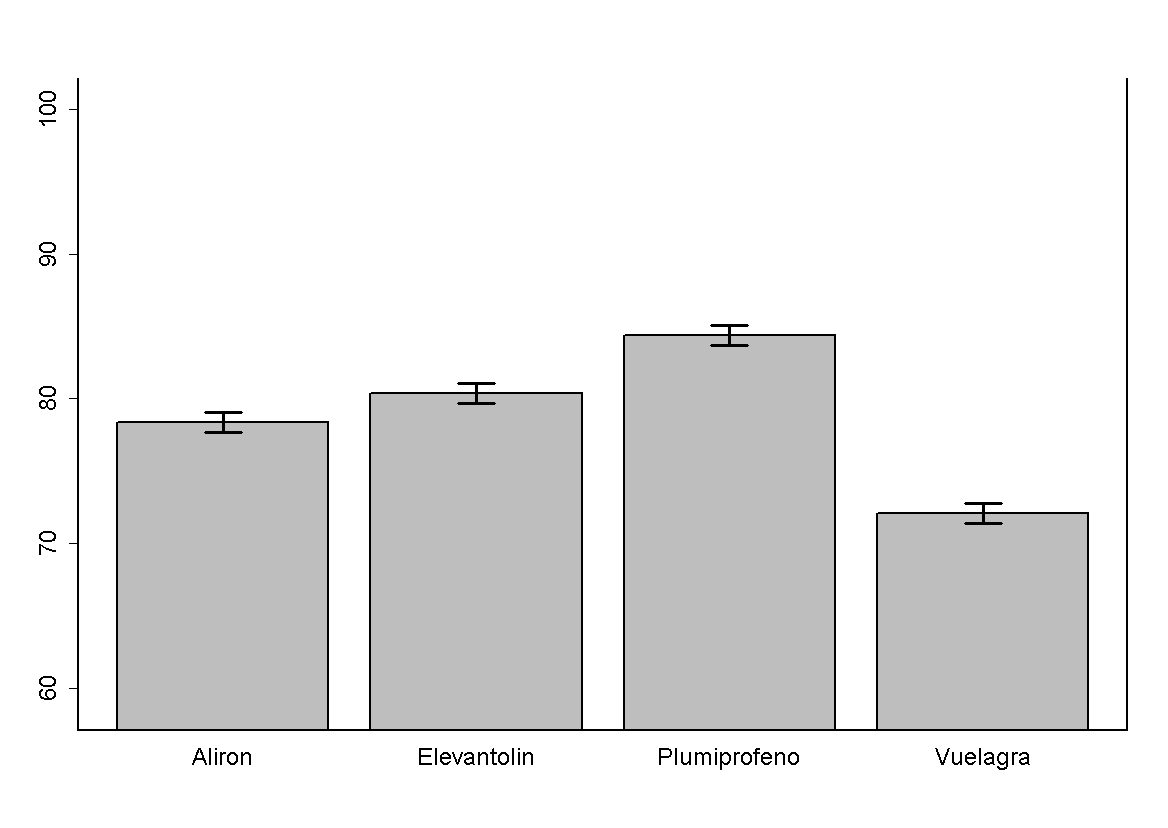
\includegraphics[width=8cm]{../fig/Tut11-04.png}
\end{center}
\caption{Diagrama de columnas con barras de error para el Ejemplo \ref{curso-cap11:ejem:Anova01} del libro.}\centering
{\bf ¡NO SE RECOMIENDA USAR ESTE TIPO DE GRÁFICOS!}
\label{tut11:fig:BargraphEjemploAnova}
\end{figure}

\begin{figure}[htb]
\begin{center}
    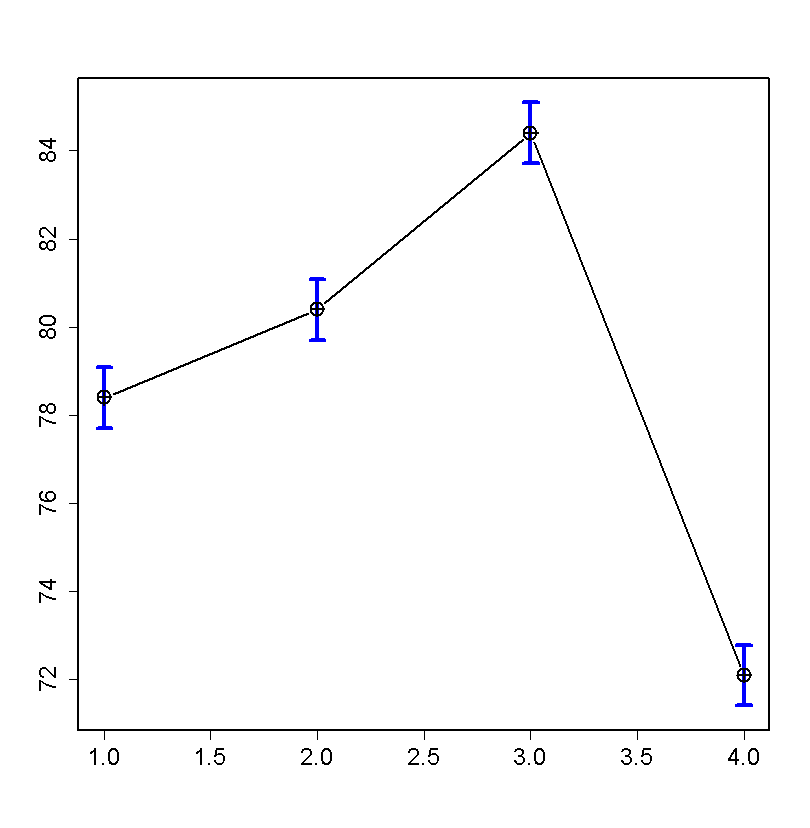
\includegraphics[width=6cm]{../fig/Tut11-05.png}
\end{center}
\caption{Un diagrama alternativo para el Ejemplo \ref{curso-cap11:ejem:Anova01} del libro.}
\label{tut11:fig:DiagramaAlternativoEjemploAnova}
\end{figure}





\section{¿Y si mis datos no están en el formato correcto?}
\label{tut11:sec:DatosFormatoNoCorrecto}

¡Ah, los placeres del {\em esquilado} de datos!

En inglés, se habla de {\sf data wrangling}, donde el {\em wrangler} es esa imagen icónica del vaquero en el rodeo, volando sobre un caballo indómito... La verdad es que no soy capaz de identificar, en el trabajo que a menudo tenemos que hacer con los datos, nada de la épica a la que supuestamente alude esa terminología en inglés. El trabajo, mucho más a menudo, me recuerda a ese otro trabajo ganadero, desde luego menos épico, que consiste en agarrar a una oveja (en general, hostil a lo que pretendemos de ella) y bregar contra el animal y su pelaje hasta reducirlo a algo mucho más aseado y presentable. Por esa razón, modestamente, propongo el uso del verbo {\em esquilar} para el tipo de operaciones que nos vamos a ver llevados a acometer demasiado a menudo.

En el caso que nos ocupa, más temprano que tarde nos tropezaremos con una tabla como la ``defectuosa'' Tabla \ref{curso-cap11:tabla:DefectuosaEjemploAnova01} (pág. \ref{curso-cap11:tabla:DefectuosaEjemploAnova01}) que hemos visto al comienzo del Capítulo \ref{curso-cap:IntroduccionAnova} del libro. Se trata de ``datos sucios'', en el sentido que hemos discutido al comienzo de este tutorial, y nos toca a nosotros la tarea de adecentarlos. No podemos ofrecerle al lector una solución general al problema, porque, por su propia esencia, los datos sucios existen en una pléyade de variantes, y no se pliegan a un tratamiento uniforme. Pero sí podemos mostrarle una estrategia que funciona, al menos en el caso de tablas como la que nos ocupa. Y, desde luego,  es un hecho constatado que se aprende con la experiencia y que, a medida que el lector se vaya encontrando en el futuro con otras dificultades, los métodos, técnicas y trucos del oficio de esquilador de datos le servirán para fabricar una solución a medida del problema.

Sin más preámbulos, vamos a presentar el fichero
\begin{center}
\fichero{./code/Tut11-Anova-EsquilandoDatos.R}{Tut11-Anova-EsquilandoDatos.R}
\end{center}
%cuyo listado aparece en la Tabla \ref{Tut07:tabla:Fichero-Tut11-Anova-FicheroEsquilarDatos}.
Las instrucciones y comentarios de ese fichero de código deberían servir de explicación suficiente del funcionamiento del fichero. Su propósito es leer un fichero de texto plano con datos (típicamente un fichero {\tt csv}), en el que se ha guardado una tabla como la Tabla \ref{curso-cap11:tabla:DefectuosaEjemploAnova01} que hemos mencionado, y producir como resultado un nuevo fichero csv con la versión ``limpia'' de esos datos, lista, por ejemplo, para usarla con los ficheros que hemos visto en las dos primeras secciones de este tutorial. Un ejemplo típico de tabla de entrada (``sucia'') puede ser este:
\begin{center}
\begin{tabular}{cccc}
Lago1&Lago2&Lago3&Lago4\\
7.1&7.2&5.6&7.2\\
8.5&6.5&7.1&6.6\\
6.2&5.9&6.3&6.3\\
7.3&7.8&6.7&7.4\\
7.9&&6.5
\end{tabular}
\end{center}

que están disponibles en el fichero
\begin{center}
\fichero{../datos/Tut11-DatosSucios.csv}{Tut11-DatosSucios.csv}
\end{center}
El aspecto más complicado de ese fichero es que es necesario contemplar la posibilidad de que, como en esta tabla, haya un número distinto de réplicas para cada uno de los niveles del tratamiento. Por eso la función {\tt read.table} incluye un argumento {\tt na.strings=c("NA"," ","")} (del inglés, {\em Not Available}), cuyo propósito es detectar las posibles formas de codificar un dato ``ausente'' en la tabla. La gestión adecuada de esos datos ausentes es, como hemos comentado en alguna otra ocasión, una de las dificultades más comunes del análisis de datos.

\section{Introducción a los contrastes con R.}
\label{tut11:sec:IntroduccionALosContrastes}
\noindent{\bf Opcional: esta sección puede omitirse en una primera lectura. }


En la Sección \ref{tut11:subsec:TablaAnovaConFuncionAnovaR} (pág. \pageref{tut11:subsec:TablaAnovaConFuncionAnovaR}) hemos usado la función {\tt lm} para obtener de manera rápida la tabla Anova del ejemplo de los frailecillos. Recordemos que esa tabla era:


\begin{knitrout}
\definecolor{shadecolor}{rgb}{0.969, 0.969, 0.969}\color{fgcolor}\begin{kframe}
\begin{verbatim}
## 
## Call:
## lm(formula = Respuesta ~ Tratamiento, data = datos)
## 
## Residuals:
##    Min     1Q Median     3Q    Max 
## -11.37  -2.81   0.11   2.77  11.11 
## 
## Coefficients:
##                         Estimate Std. Error t value Pr(>|t|)    
## (Intercept)               78.399      0.420  186.68  < 2e-16 ***
## TratamientoElevantolin     2.000      0.594    3.37  0.00083 ***
## TratamientoPlumiprofeno    6.001      0.594   10.10  < 2e-16 ***
## TratamientoVuelagra       -6.299      0.594  -10.61  < 2e-16 ***
## ---
## Signif. codes:  0 '***' 0.001 '**' 0.01 '*' 0.05 '.' 0.1 ' ' 1
## 
## Residual standard error: 4.2 on 396 degrees of freedom
## Multiple R-squared:  0.531,	Adjusted R-squared:  0.527 
## F-statistic:  149 on 3 and 396 DF,  p-value: <2e-16
\end{verbatim}
\end{kframe}
\end{knitrout}

En aquella sección vimos que el primer valor que aparece en la fila {\tt Intercept} es la media $\bar X_{{\mbox{\bf\large$\cdot$}}1}=78.40$ del primer nivel (por orden alfabético), el {\em Aliron}. Los valores iniciales de las siguientes tres filas son {\em las diferencias} entre este valor y las medias de los restantes tres niveles:
\[
\begin{cases}
\bar X_{{\mbox{\bf\large$\cdot$}}2} - \bar X_{{\mbox{\bf\large$\cdot$}}1} =  80.40 - 78.40 = 2.00\\
\bar X_{{\mbox{\bf\large$\cdot$}}3} - \bar X_{{\mbox{\bf\large$\cdot$}}1} =  84.40 - 78.40 = 6.00\\
\bar X_{{\mbox{\bf\large$\cdot$}}4} - \bar X_{{\mbox{\bf\large$\cdot$}}1} =  72.10 - 78.40 = -6.30\\
\end{cases}
\]
También dijimos entonces que íbamos a tratar de entender por qué nos pueden interesar estos valores, y qué significan las restantes columnas de la tabla en la que aparecen. Además,  en esta sección vamos a aprender a controlar el proceso, para que los cálculos de R se ajusten a nuestros deseos en una situación experimental concreta.

A la vista de la tabla está claro que:
\begin{itemize}
  \item Los coeficientes de la primera columna están relacionados con los coeficientes $b_0, b_1,\ldots, b_4$ del modelo lineal Anova que aparecen en el Ejemplo \ref{curso-cap11:ejem:EstimacionFrailecillosModeloLineal} del libro (pág. \pageref{curso-cap11:ejem:EstimacionFrailecillosModeloLineal}). Por ejemplo,
  $$b_2 - b_1 = \left(\bar X_{{\mbox{\bf\large$\cdot$}}2}-b_0\right) - \left(\bar X_{{\mbox{\bf\large$\cdot$}}1}- b_0\right) = \bar X_{{\mbox{\bf\large$\cdot$}}2} - \bar X_{{\mbox{\bf\large$\cdot$}}1}$$
  \item La suma de los coeficientes $b_1, b_2, b_3, b_4$ es igual a $0$, por su propia definición (y si en el el Ejemplo \ref{curso-cap11:ejem:EstimacionFrailecillosModeloLineal} la suma {\em parece} no ser cero es por los efectos del redondeo). En términos prácticos, eso significa que uno de esos coeficientes {\em sobra, está de más}. No aporta ninguna información que no podamos extraer de los restantes. En la Sección \ref{tut11:sec:IntroduccionALosContrastes} del Tutorial veremos que la forma en la que R ha expresado el modelo tiene, entre otras, la virtud de que {\em no hay coeficientes de sobra}. Por eso la tabla {\tt Coefficients} en la salida de {\tt summary(datos.lm)} tiene sólo cuatro filas, mientras que $b_0, \ldots, b_4$ son cinco coeficientes.
\end{itemize}

La idea clave para controlar la información que aparece en la tabla Anova es la noción de contraste que se discute en la Sección \ref{curso-cap11:subsubsec:IntroduccionContrastes} del libro (pág. \pageref{curso-cap11:subsubsec:IntroduccionContrastes}). Vamos a aprender cómo usa R esos contratses y, en particular, cómo definir nuestros propios contrastes. Pero para llegar hasta ahí el primer paso es entender en detalle la noción de variables {\em dummy} que hemos visto en la página \pageref{curso-cap11:subsubsec:VariablesDummy} del libro.

\subsubsection*{Variables dummy en R, construcción a mano.}
\label{tut11:subsubsec:VariablesDummyEnRaMano}


Al leer la Sección \ref{curso-cap11:subsec:AnovaComoModeloLineal} del libro (pág. \pageref{curso-cap11:subsec:AnovaComoModeloLineal}) es posible que te hayas preguntado cómo construir en R esas variables índice (o variables {\em dummy}) que hemos utilizado para expresar Anova como un modelo lineal. Lo primero que queremos apresurarnos a decir es que en realidad no es necesario hacer esto: las variables de tipo {\tt factor} de R sirven, entre otras cosas, para que no tengamos que ocuparnos de crear estas variables índice manualmente. Podemos relajarnos y dejar que R se encargue de ese trabajo por nosotros.

Pero, como suele suceder, mientras uno está aprendiendo a hacer algo por primera vez, esa construcción manual puede ayudar a entender lo que estamos haciendo. Es una situación parecida a la construcción manual de la tabla Anova que hemos hecho antes. Por supuesto, los profesionales usan siempre {\tt lm} para obtener esa tabla. Pero es bueno, pedagógicamente, construirla a mano las primeras veces. Una de las razones por las que nos gustan las herramientas como R es que, a diferencia de soluciones tipo {\em caja negra}, permiten hacer ese tipo de construcciones manuales con tanto detalle como se desee. Además, como hemos dicho, entender las variables dummy nos va a facilitar mucho la tarea de entender como se gestionan los contrastes en R.

Manos a la obra entonces. Vamos a construir las variables $T_1, T_2, T_3, T_4$ del Ejemplo \ref{curso-cap11:ejem:TablaVariablesIndicadoras} del libro (pág. \pageref{curso-cap11:ejem:TablaVariablesIndicadoras}). La idea es muy sencilla: para definir, por ejemplo, una variable {\tt T1} que valga 1 en los frailecillos tratado scon el primer tratamiento ({\em Alirón}) basta con usar este código:
\begin{knitrout}
\definecolor{shadecolor}{rgb}{0.969, 0.969, 0.969}\color{fgcolor}\begin{kframe}
\begin{alltt}
\hlstd{T1}  \hlkwb{=} \hlkwd{as.integer}\hlstd{(datos}\hlopt{$}\hlstd{Tratamiento} \hlopt{==} \hlstr{"Aliron"}\hlstd{)}
\end{alltt}
\end{kframe}
\end{knitrout}
Hemos usado la función {\tt as.integer} para convertor los valores booleanos {\tt TRUE/FALSE} en $0$s y $1$s. Ya sabes que R los gestiona así directamente, pero esta vez queríamos hacer explícita la codificación numérica. Un inconveniente de este código es que depende del nombre concreto de ese nivel. Podemos hacerlo mejor definiendo así las  variables índice:
\begin{knitrout}
\definecolor{shadecolor}{rgb}{0.969, 0.969, 0.969}\color{fgcolor}\begin{kframe}
\begin{alltt}
\hlcom{### Variables indice}

\hlstd{T1}  \hlkwb{=} \hlkwd{as.integer}\hlstd{(datos}\hlopt{$}\hlstd{Tratamiento} \hlopt{==} \hlkwd{levels}\hlstd{(datos}\hlopt{$}\hlstd{Tratamiento)[}\hlnum{1}\hlstd{])}
\hlstd{T2}  \hlkwb{=} \hlkwd{as.integer}\hlstd{(datos}\hlopt{$}\hlstd{Tratamiento} \hlopt{==} \hlkwd{levels}\hlstd{(datos}\hlopt{$}\hlstd{Tratamiento)[}\hlnum{2}\hlstd{])}
\hlstd{T3}  \hlkwb{=} \hlkwd{as.integer}\hlstd{(datos}\hlopt{$}\hlstd{Tratamiento} \hlopt{==} \hlkwd{levels}\hlstd{(datos}\hlopt{$}\hlstd{Tratamiento)[}\hlnum{3}\hlstd{])}
\hlstd{T4}  \hlkwb{=} \hlkwd{as.integer}\hlstd{(datos}\hlopt{$}\hlstd{Tratamiento} \hlopt{==} \hlkwd{levels}\hlstd{(datos}\hlopt{$}\hlstd{Tratamiento)[}\hlnum{4}\hlstd{])}
\end{alltt}
\end{kframe}
\end{knitrout}
Por lo demás, si fuéramos a escribir un código general para este tipo de operaciones deberíamos además escribirlo de forma que el código se adaptara de forma automática al número de niveles del factor tratamiento. Pero como sólo estamos haciendo un experimento nos vamos a conformar con el anterior método para definir las $T_i$.

Podemos añadir estas variables al {\tt data.frame} con los datos usando {\tt cbind}, como si fuera una matriz:
\begin{knitrout}
\definecolor{shadecolor}{rgb}{0.969, 0.969, 0.969}\color{fgcolor}\begin{kframe}
\begin{alltt}
\hlstd{datos} \hlkwb{=} \hlkwd{cbind}\hlstd{(datos, T1, T2, T3, T4)}
\end{alltt}
\end{kframe}
\end{knitrout}
Y si observamos las primeras 10 filas de los datos veremos que las variables índice que hemos construido hacen exactamente lo que esperábamos de ellas:
\begin{knitrout}
\definecolor{shadecolor}{rgb}{0.969, 0.969, 0.969}\color{fgcolor}\begin{kframe}
\begin{alltt}
\hlkwd{head}\hlstd{(datos,} \hlnum{10}\hlstd{)}
\end{alltt}
\begin{verbatim}
##     Tratamiento Respuesta T1 T2 T3 T4
## 1        Aliron     76.65  1  0  0  0
## 2   Elevantolin     88.66  0  1  0  0
## 3        Aliron     79.36  1  0  0  0
## 4      Vuelagra     76.74  0  0  0  1
## 5        Aliron     71.83  1  0  0  0
## 6      Vuelagra     74.72  0  0  0  1
## 7  Plumiprofeno     87.14  0  0  1  0
## 8        Aliron     73.24  1  0  0  0
## 9   Elevantolin     78.12  0  1  0  0
## 10 Plumiprofeno     82.34  0  0  1  0
\end{verbatim}
\end{kframe}
\end{knitrout}

Es importante entender que estas variables índice contienen exactamente la misma información que la variable {\tt Tratamiento}, pero codificada de otra manera. Antes, para construir el modelo lineal del Anova hemos usado la función {\tt lm} con esta fórmula:
\begin{knitrout}
\definecolor{shadecolor}{rgb}{0.969, 0.969, 0.969}\color{fgcolor}\begin{kframe}
\begin{alltt}
\hlstd{datos.lm} \hlkwb{=} \hlkwd{lm}\hlstd{(Respuesta} \hlopt{~} \hlstd{Tratamiento,} \hlkwc{data} \hlstd{= datos)}
\end{alltt}
\end{kframe}
\end{knitrout}
Pero, puesto que las variables índice contienen la misma información que {\tt Tratamiento}, podemos usarlas como variables predictoras para construir el modelo. No podemos entrar en todos los detalles aquí, ni mucho menos, porque eso supondría adentrarnos en el terreno de los modelos con más de una variable predictora. Pero podemos decir que cuando se usan estos modelos en R, la forma más sencilla de indicar que hay varias variables en el modelo es separándolas con el símbolo {\tt +}, como hemos hecho en este nuevo intento de construir el modelo:

\begin{knitrout}
\definecolor{shadecolor}{rgb}{0.969, 0.969, 0.969}\color{fgcolor}\begin{kframe}
\begin{alltt}
\hlstd{(datos.lm2} \hlkwb{=} \hlkwd{lm}\hlstd{(Respuesta} \hlopt{~} \hlstd{T1} \hlopt{+} \hlstd{T2} \hlopt{+} \hlstd{T3} \hlopt{+} \hlstd{T4,} \hlkwc{data} \hlstd{= datos))}
\end{alltt}
\begin{verbatim}
## 
## Call:
## lm(formula = Respuesta ~ T1 + T2 + T3 + T4, data = datos)
## 
## Coefficients:
## (Intercept)           T1           T2           T3           T4  
##        72.1          6.3          8.3         12.3           NA
\end{verbatim}
\end{kframe}
\end{knitrout}

De nuevo una pregunta parecida a la de antes: ¿qué son esos cinco coeficientes? La situación se ve agravada además por el hecho de que uno de ellos es {\tt NA}. El problema se debe, como hemos señalado, al hecho de que estamos tratando de usar cuatro variables explicativas {\em que no son independientes}; sobra una de ellas. Si sabes algo de Álgebra Lineal, la situación es similar a  tratar de resolver un sistema de ecuaciones lineales en el que la matriz de coeficientes tiene determinante cero: lo normal es que tengamos problemas para hacerlo. R, en este caso, al constatar que sobraban variables ha tomado como término independiente del modelo la media del cuarto nivel del tratamiento, $\bar X_{{\mbox{\bf\large$\cdot$}}4}\approx 72.1$ y ha trabajado con una ecuación del modelo de la forma:
$$X=c_0 + c_1 \cdot T^{(1)} + c_2 \cdot T^{(2)} + c_3 \cdot T^{(3)}$$
en la que además,
$$
\begin{cases}
c_0 = \bar X_{{\mbox{\bf\large$\cdot$}}4}\approx72.1\\
c_1 = \bar X_{{\mbox{\bf\large$\cdot$}}1} - \bar X_{{\mbox{\bf\large$\cdot$}}4}\approx6.299\\
c_2 = \bar X_{{\mbox{\bf\large$\cdot$}}2} - \bar X_{{\mbox{\bf\large$\cdot$}}4}\approx8.3\\
c_3 = \bar X_{{\mbox{\bf\large$\cdot$}}3} - \bar X_{{\mbox{\bf\large$\cdot$}}4}\approx12.3\\
\end{cases}
$$
En este caso hemos dejado que R, al comprobar que sobran variables explicativas, eligiera cuál de esas variables se eliminaba. Podemos controlar un poco más el proceso, eligiendo nosotros mismos una de las variables índice para descartarla y construir el modelo a partir de las restantes. Por ejemplo, si decidimos descartar {\tt T1}, entonces hacemos:
\begin{knitrout}
\definecolor{shadecolor}{rgb}{0.969, 0.969, 0.969}\color{fgcolor}\begin{kframe}
\begin{alltt}
\hlstd{(datos.lm3} \hlkwb{=} \hlkwd{lm}\hlstd{(Respuesta} \hlopt{~} \hlstd{T2} \hlopt{+} \hlstd{T3} \hlopt{+} \hlstd{T4,} \hlkwc{data} \hlstd{= datos))}
\end{alltt}
\begin{verbatim}
## 
## Call:
## lm(formula = Respuesta ~ T2 + T3 + T4, data = datos)
## 
## Coefficients:
## (Intercept)           T2           T3           T4  
##        78.4          2.0          6.0         -6.3
\end{verbatim}
\end{kframe}
\end{knitrout}
Si ahora comparas estos resultados con los que obtuvimos al usar inicialmente {\tt lm} así:
\begin{knitrout}
\definecolor{shadecolor}{rgb}{0.969, 0.969, 0.969}\color{fgcolor}\begin{kframe}
\begin{alltt}
\hlstd{datos.lm} \hlkwb{=} \hlkwd{lm}\hlstd{(Respuesta} \hlopt{~} \hlstd{Tratamiento,} \hlkwc{data} \hlstd{= datos)}
\end{alltt}
\end{kframe}
\end{knitrout}
y que, recordémoslo, eran:
\begin{knitrout}
\definecolor{shadecolor}{rgb}{0.969, 0.969, 0.969}\color{fgcolor}\begin{kframe}
\begin{alltt}
\hlstd{datos.lm}\hlopt{$}\hlstd{coefficients}
\end{alltt}
\begin{verbatim}
##             (Intercept)  TratamientoElevantolin TratamientoPlumiprofeno 
##                 78.3993                  2.0004                  6.0008 
##     TratamientoVuelagra 
##                 -6.2994
\end{verbatim}
\end{kframe}
\end{knitrout}
parece que hemos empezado a entender la respuesta inicial de R. Decimos que hemos empezado a entenderla porque el contexto natural de esta discusión es el lenguaje de contrastes.

% que se discuten en la Sección \ref{curso-cap11:subsubsec:IntroduccionContrastes} del libro (pág. \pageref{curso-cap11:subsubsec:IntroduccionContrastes}) y sobre los que, en este tutorial, hablaremos en la Sección \ref{tut11:sec:IntroduccionALosContrastes}.

\subsection{Contrastes en R.}
\label{tut11:subsec:ContrastesEnR}

En la Sección \ref{curso-cap11:subsubsec:IntroduccionContrastes} del libro (pág. \pageref{curso-cap11:subsubsec:IntroduccionContrastes}) hemos visto que la técnica de los {\em contrastes} puede usarse como forma de adaptar el método Anova a algunas peculiaridades de nuestro diseño experimental. Por ejemplo en presencia de un grupo (nivel) especial de tratamiento que queremos comparar con los demás. Los {\em contrastes} son también una respuesta al problema de la dependencia de las variables índice ({\em dummy}).

Con R es muy fácil usar este método. Empecemos recordando que en la práctica un contraste se define mediante una combinación lineal de las medias de los distintos niveles del factor
$$a_1\cdot\mu_1+a_1\cdot\mu_1+\cdots+a_k\cdot\mu_k$$
con la condición de que la suma de los coeficientes $a_i$ es igual a $0$:
\[a_1+a_2+\cdots+a_k=0.\]
Para usarlos en un contraste tipo Anova debemos seleccionar una colección de $k-1$ contrastes independientes, identificados mediante una matriz. Cuando usamos la función {\tt lm} para hacer un contraste Anova, R  selecciona por defecto una cierta {\em matriz de contrastes}. Para ver cuál es esa matriz vamos a empezar usando este comando:
\begin{knitrout}
\definecolor{shadecolor}{rgb}{0.969, 0.969, 0.969}\color{fgcolor}\begin{kframe}
\begin{alltt}
\hlkwd{contrasts}\hlstd{(datos}\hlopt{$}\hlstd{Tratamiento)}
\end{alltt}
\begin{verbatim}
##              Elevantolin Plumiprofeno Vuelagra
## Aliron                 0            0        0
## Elevantolin            1            0        0
## Plumiprofeno           0            1        0
## Vuelagra               0            0        1
\end{verbatim}
\end{kframe}
\end{knitrout}
Esta no es todavía la matriz de contrastes, pero está estrechamente relacionada con ella. ¿Qué representa esta matriz, cómo se interpretan esos números? Para entenderlo, vamos a recordar que, como hemos visto en la Sección \ref{curso-cap11:subsubsec:IntroduccionContrastes}, hay dos formas de caracterizar un conjunto de contrastes. Una es mediante la {\em matriz del contraste} $M$ que interviene en:
\[
\left(
\begin{array}{c}
\alpha_1\\\alpha_2\\\vdots\\\alpha_k
\end{array}
\right)
=
\left(
\begin{array}{cccc}
a_{1,1}&a_{1,2}&\cdots&a_{1,k}\\
a_{2,1}&a_{2,2}&\cdots&a_{2,k}\\
&&\ddots&\\
a_{k,1}&a_{k,2}&\cdots&a_{k,k}\\
\end{array}
\right)
\cdot
\left(
\begin{array}{c}
\mu_1\\\mu_2\\\vdots\\\mu_k
\end{array}
\right)
\]
La otra es mediante su inversa $M^{-1}$, que es la más cómoda cuando se trata de construir las variables índice asociadas a ese conjunto de contrastes. La matriz que se obtiene con {\tt contrasts} está relacionada con esa inversa $M^{-1}$ y eso hace que, al principio, sea un poco más difícil reconocer el conjunto de contrastes que está usando R. Para obtener la matriz de contrastes, como hemos argumentado en el libro (ver pág. \pageref{curso-cap11:subsubsec:MatrizContrastesModelo}), tenemos que añadir a la izquierda una columna de unos y calcular la inversa de la matriz resultante. En R la inversa de una matriz se calcula con {\tt solve} (ver el Tutorial03):
\begin{knitrout}
\definecolor{shadecolor}{rgb}{0.969, 0.969, 0.969}\color{fgcolor}\begin{kframe}
\begin{alltt}
\hlstd{(Minversa} \hlkwb{=} \hlkwd{cbind}\hlstd{(}\hlkwd{rep}\hlstd{(}\hlnum{1}\hlstd{, k),}\hlkwd{contrasts}\hlstd{(datos}\hlopt{$}\hlstd{Tratamiento)))}
\end{alltt}
\begin{verbatim}
##                Elevantolin Plumiprofeno Vuelagra
## Aliron       1           0            0        0
## Elevantolin  1           1            0        0
## Plumiprofeno 1           0            1        0
## Vuelagra     1           0            0        1
\end{verbatim}
\begin{alltt}
\hlstd{(M} \hlkwb{=} \hlkwd{solve}\hlstd{(Minversa))}
\end{alltt}
\begin{verbatim}
##              Aliron Elevantolin Plumiprofeno Vuelagra
##                   1           0            0        0
## Elevantolin      -1           1            0        0
## Plumiprofeno     -1           0            1        0
## Vuelagra         -1           0            0        1
\end{verbatim}
\end{kframe}
\end{knitrout}
Esta última matriz $M$ es la que en el libro hemos llamado la matriz del contraste. Y, ahora sí, nos permite ver claramente el conjunto de contrastes  queR ha decidido usar:

\[
{\small
\left\{
\begin{array}{l}
\alpha_1=\mu_1,\\[1mm]
\alpha_2=\mu_2-\mu_1,\\[1mm]
\alpha_3=\mu_3-\mu_1,\\[1mm]
\alpha_4=\mu_4-\mu_1.
\end{array}\right.}
\Rightarrow
M=\left(
\begin{array}{rrrr}
1&0&0&0\\
-1&1&0&0\\
-1&0&1&0\\
-1&0&0&1
\end{array}
\right)
\]

¿Por qué este conjunto? Porque la opción por defecto consiste en suponer que queremos comparar un {\em nivel especial} frente a todos los demás niveles. Por ejemplo puede ser un placebo que se compara con varios tratamientos, o un tratamiento ya establecido frente a varias alternativas nuevas o viceversa, etc. Y a  falta de más información, R usa como {\em nivel especial} el primer nivel (que, en este caso, es {\em Alirón} porque los niveles se han ordenado alfabéticamente).

Para completar la información, R va a usar 3 variables índice, a las que vamos a llamar
$\tilde{T}^{(1)}$, $\tilde{T}^{(2)}$ y $\tilde{T}^{(3)}$ (R las nombra como algunos de los tratamientos por razones que después quedarán claras),
y que se definen mediante una tabla, cuyas columnas son las tres últimas columnas de $M^{-1}$:
\begin{center}
\begin{tabular}{l|c|c|c|}
\cline{2-4}
            \rule{0mm}{5mm}   & $\tilde{T}^{(1)}$&$\tilde{T}^{(3)}$&$\tilde{T}^{(4)}$ \\
\cline{2-4}
\mbox{Alirón:}&0&0&0 \\
\cline{2-4}
\mbox{Elevantolín:}&1&0&0 \\
\cline{2-4}
\mbox{Plumiprofeno:}&0&1&0 \\
\cline{2-4}
\mbox{Vuelagra:}&0&0&1 \\
\cline{2-4}
\end{tabular}
\end{center}
Como hemos dicho, la tabla que define estas variables índice es precisamente la matriz que se obtiene usando {\tt contrasts(datos\$Tratamiento)}.

\subsubsection*{Interpretación de los resultados de {\tt lm}.}
\label{tut11:subsubsec:InterpretacionResultadosLm}

Ahora que ya sabemos cuál es el conjunto de contrastes que R ha decidido usar estamos listos para entender con más detalle lo que se obtiene al usar la función {\tt lm}, un trabajo que habíamos dejado pendiente desde el principio de la Sección \ref{tut11:subsec:TablaAnovaConFuncionAnovaR} (pág. \pageref{tut11:subsec:TablaAnovaConFuncionAnovaR}).

\begin{knitrout}
\definecolor{shadecolor}{rgb}{0.969, 0.969, 0.969}\color{fgcolor}\begin{kframe}
\begin{alltt}
\hlkwd{summary}\hlstd{(}\hlkwd{lm}\hlstd{(datos}\hlopt{$}\hlstd{Respuesta} \hlopt{~} \hlstd{datos}\hlopt{$}\hlstd{Tratamiento))}
\end{alltt}
\begin{verbatim}
## 
## Call:
## lm(formula = datos$Respuesta ~ datos$Tratamiento)
## 
## Residuals:
##    Min     1Q Median     3Q    Max 
## -11.37  -2.81   0.11   2.77  11.11 
## 
## Coefficients:
##                               Estimate Std. Error t value Pr(>|t|)    
## (Intercept)                     78.399      0.420  186.68  < 2e-16 ***
## datos$TratamientoElevantolin     2.000      0.594    3.37  0.00083 ***
## datos$TratamientoPlumiprofeno    6.001      0.594   10.10  < 2e-16 ***
## datos$TratamientoVuelagra       -6.299      0.594  -10.61  < 2e-16 ***
## ---
## Signif. codes:  0 '***' 0.001 '**' 0.01 '*' 0.05 '.' 0.1 ' ' 1
## 
## Residual standard error: 4.2 on 396 degrees of freedom
## Multiple R-squared:  0.531,	Adjusted R-squared:  0.527 
## F-statistic:  149 on 3 and 396 DF,  p-value: <2e-16
\end{verbatim}
\end{kframe}
\end{knitrout}

Concretamente, empecemos por la columna {\tt Estimate} de la tabla {\tt Coefficients}. Recuerda que el modelo Anova que R está usando (el que elige por defecto) es:
$$X = \alpha_0 + c_1 \cdot T^{(1)} + c_2 \cdot T^{(2)} + c_3 \cdot T^{(3)} + \varepsilon$$
donde los $\alpha_i$ son los contrastes que hemos visto:
$$\alpha_1=\mu_1,\quad \alpha_2=\mu_2-\mu_1,\quad \alpha_3=\mu_3-\mu_1,\quad \alpha_4=\mu_4-\mu_1$$
Los valores {\tt Estimate} son las estimaciones que R ha obtenido de los valores de los $\alpha$. Y debería ser evidente que, por ejemplo, la estimación de $\alpha_3= \mu_3 - \mu_1$ sólo puede ser $\bar X_{\mbox{\bf\large $\cdot$}3} - \bar X_{\mbox{\bf\large $\cdot$}1}$. Comprobémoslo para  todos los $\alpha_i$ (el caso de $\alpha_1$ es especial, por eso lo hemos separado de los demás):

\begin{knitrout}
\definecolor{shadecolor}{rgb}{0.969, 0.969, 0.969}\color{fgcolor}\begin{kframe}
\begin{alltt}
\hlstd{alphas} \hlkwb{=} \hlkwd{summary}\hlstd{(datos.lm)}\hlopt{$}\hlstd{coefficients[,} \hlnum{1}\hlstd{]}

\hlstd{alphas[}\hlnum{1}\hlstd{]}
\end{alltt}
\begin{verbatim}
## (Intercept) 
##      78.399
\end{verbatim}
\begin{alltt}
\hlstd{mediasPorNivel[}\hlnum{1}\hlstd{]}
\end{alltt}
\begin{verbatim}
## Aliron 
## 78.399
\end{verbatim}
\begin{alltt}
\hlstd{alphas[}\hlnum{2}\hlopt{:}\hlnum{4}\hlstd{]}
\end{alltt}
\begin{verbatim}
##  TratamientoElevantolin TratamientoPlumiprofeno     TratamientoVuelagra 
##                  2.0004                  6.0008                 -6.2994
\end{verbatim}
\begin{alltt}
\hlstd{mediasPorNivel[}\hlnum{2}\hlopt{:}\hlnum{4}\hlstd{]} \hlopt{-} \hlstd{mediasPorNivel[}\hlnum{1}\hlstd{]}
\end{alltt}
\begin{verbatim}
##  Elevantolin Plumiprofeno     Vuelagra 
##       2.0004       6.0008      -6.2994
\end{verbatim}
\end{kframe}
\end{knitrout}
Como esperábamos, las estimaciones coinciden con las correspondientes diferencias de medias por niveles.  Ahora podemos entender el resto de las columnas de esa tabla {\tt Coefficients}. Lo que queremos saber, cuando utilizamos un cierto conjunto de contrastes, es cuáles de ellos son significativos. Por ejemplo, al usar el contraste $\alpha_2 =\mu_2-\mu_1$, si ese contraste resulta significativo podremos concluir que hay una diferencia significativa entre las medias de los niveles 1 y 2 del tratamiento. Es decir, que la  hipótesis nula que estamos contrastando con el contraste $\alpha_2$ es:
$$H_0 = \{\alpha_2 = \mu_2-\mu_1 = 0\}$$
El estadístico que necesitamos para este contraste (contraste de hipótesis sobre el contraste $\alpha_2$, la terminología es así de confusa...) aparece en la Ecuación \ref{curso-cap11:ecu:EstadisticoContrasteIgualCero} del libro (pág. \pageref{curso-cap11:ecu:EstadisticoContrasteIgualCero}).
\[
\Xi=\dfrac{
                \left(\sum_{j=1}^{k}a_j\cdot\bar X_{\mbox{\bf\large $\cdot$}j}\right)
                -
                \left(\sum_{j=1}^{k}a_j\cdot\mu_j\right)
             }{
             \sqrt{s^2_{\mbox{pond}}\cdot
                \sum_{j=1}^{k}\dfrac{a_j^2}{n_j}
             }
             }
\]
donde $s_{\mbox{pond}}^2$ es la {\em cuasidesviación ponderada} (en inglés, {\em pooled sd}), que ya hemos calculado antes para usarla en el ajuste de Bonferroni  y que hemos guardado en la variable {\tt poolesSd} de R. Vamos a calcular entonces el estadístico $\Xi$ para el contraste $\alpha_2=\mu_2-\mu_1$. Para hacerlo necesitamos además los valores $n_k$, el número de observaciones en cada nivel del factor, que hemos almacenado en el vector {\tt replicas} (ver el bloque de {\em Construcción manual de la tabla Anova} en el fichero {\tt Tut11-Anova-Basico.R}).

\begin{knitrout}
\definecolor{shadecolor}{rgb}{0.969, 0.969, 0.969}\color{fgcolor}\begin{kframe}
\begin{alltt}
\hlstd{(numerEstad} \hlkwb{=} \hlkwd{t}\hlstd{(mediasPorNivel)} \hlopt \hlstd{M[}\hlnum{2}\hlstd{, ])}
\end{alltt}
\begin{verbatim}
##        [,1]
## [1,] 2.0004
\end{verbatim}
\begin{alltt}
\hlstd{(denomEstad} \hlkwb{=} \hlstd{pooledSd} \hlopt{*} \hlkwd{sqrt}\hlstd{(}\hlkwd{sum}\hlstd{(M[}\hlnum{2}\hlstd{, ]}\hlopt{^}\hlnum{2} \hlopt{/} \hlstd{replicas)))}
\end{alltt}
\begin{verbatim}
## [1] 0.59393
\end{verbatim}
\begin{alltt}
\hlstd{(Estadistico} \hlkwb{=} \hlstd{numerEstad} \hlopt{/} \hlstd{denomEstad)}
\end{alltt}
\begin{verbatim}
##        [,1]
## [1,] 3.3681
\end{verbatim}
\end{kframe}
\end{knitrout}
Para entender esto necesitamos un poco de álgebra lineal. Hemos usado el producto matricial \verb# %*% #
del vector fila {\tt t(mediasPorNivel)} por la segunda fila de la matriz de contrastes, para calcular el numerador del estadístico. Si sabes algo de álgebra, también puedes verlo como el producto escalar de los vectores $(a_1,\ldots,a_j)$ y $(\bar X_{{\mbox{\bf\large$\cdot$}}1},\ldots,\bar X_{{\mbox{\bf\large$\cdot$}}j})$

Este valor del estadístico aparece en la segunda fila de la columna titulada {\tt t value} de la tabla {\tt Coefficients}. Es la segunda fila porque estamos trabajando con el contraste  $\alpha_2$, claro. Y ahora podemos usar la distribución $t$ de Student adecuada, con $N - k$ grados de libertad, para calcular el p-valor del contraste de hipótesis sobre el contraste $\alpha_2$. Tengamos en cuenta que la hipótesis nula que estamos contrastando es:
$$H_0 = \{\alpha_2 =0\}$$
así que se trata de un contraste bilateral:
\begin{knitrout}
\definecolor{shadecolor}{rgb}{0.969, 0.969, 0.969}\color{fgcolor}\begin{kframe}
\begin{alltt}
\hlstd{(pValor} \hlkwb{=} \hlnum{2} \hlopt{*} \hlstd{(}\hlnum{1} \hlopt{-} \hlkwd{pt}\hlstd{(}\hlkwd{abs}\hlstd{(Estadistico),} \hlkwc{df}\hlstd{=N}\hlopt{-}\hlstd{k)))}
\end{alltt}
\begin{verbatim}
##            [,1]
## [1,] 0.00083106
\end{verbatim}
\end{kframe}
\end{knitrout}
y puedes comprobar que el resultado coincide con lo que aparece en la segunda fila de la última columna de la tabla {\tt Coefficients}, titulada {\tt Pr(>|t|)}. Por cierto, la segunda columna de esa tabla contiene, en sus tres últimas filas, el valor que nosotros hemos llamado {\tt denomEstad}.

\begin{ejercicio}
\label{tut11:ejercicio07}
Comprueba, igual que hemos hecho aquí, el resto de valores de la tabla {\tt Coefficients}.
% Soluciones en la página \pageref{tut11:ejercicio07:sol}.
\qed
\end{ejercicio}


\subsubsection*{Contrastes definidos por el usuario.}
\label{tut11:subsubsec:ContrastesDefinidosPorElUsuario}

Acabamos de ver que cuando usamos la función {\tt lm} para hacer un contraste Anova,  R utiliza por defecto un cierto conjunto de contrastes. Concretamente, si tenemos $k$ niveles del tratamiento, sean $T_1, T_2, \ldots, T_k$, con medias respectivas $\mu_1, \mu_2,\ldots, \mu_k$, entonces R usa:
\[
\begin{cases}
\alpha_2=\mu_2-\mu_1,\\
\alpha_3=\mu_3-\mu_1,\\
\quad\vdots\\
\alpha_k=\mu_k-\mu_1.
\end{cases}
\]
donde, como ya sabemos,  $\alpha_1$ no es un contraste. Este conjunto de contrastes es adecuado si consideramos que el nivel $T_1$ es especial en algún sentido y  queremos compararlo con todos los restantes grupos. Pero hay muchas otras situaciones imaginables, que aparecen con frecuencia en el trabajo de los investigadores. Para dar cabida a esos objetivos experimentales, R pone a nuestra disposición la posibilidad de crear nuestra propia matriz de contrastes. Vamos a ver un ejemplo de cómo se hace esto.

Para empezar, vamos a fijar el objetivo que nos hemos planteado. En muchas ocasiones, los investigadores tienen una idea previa de cómo se ordenan las medias de  los niveles del tratamiento. Imagínate que en nuestro ejemplo de los frailecillos, un investigador sospecha que la ordenación de las medias es esta:
$$\mu_4 < \mu_1 < \mu_3 < \mu_2$$
Otra forma de expresar esto es
$$0 < \mu_1 - \mu_4, \quad  0 < \mu_3 - \mu_1, \quad 0 < \mu_2 - \mu_3.$$
Para comprobar estas ideas, podemos diseñar esta colección de contrastes:
$$
\begin{cases}
\alpha_2 = \mu_1 - \mu_4\\
\alpha_3 = \mu_3 - \mu_1\\
\alpha_4 = \mu_2 - \mu_3\\
\end{cases}
$$
Añadimos este término independiente:
$$\alpha_1 = \mu_4$$
¿Por qué elegimos este término independiente? Volveremos sobre esto enseguida. La matriz de este conjunto de contrastes es:
$$M=\left(
\begin{array}{rrrr}
0&0&0&1\\
1&0&0&-1\\
-1&0&1&0\\
0&1&-1&0
\end{array}
\right)$$
En R esto es:
\begin{knitrout}
\definecolor{shadecolor}{rgb}{0.969, 0.969, 0.969}\color{fgcolor}\begin{kframe}
\begin{alltt}
\hlstd{(M} \hlkwb{=} \hlkwd{matrix}\hlstd{(}\hlkwd{c}\hlstd{(}\hlnum{0}\hlstd{,} \hlnum{0}\hlstd{,} \hlnum{0}\hlstd{,} \hlnum{1}\hlstd{,} \hlnum{1}\hlstd{,} \hlnum{0}\hlstd{,} \hlnum{0}\hlstd{,} \hlopt{-}\hlnum{1}\hlstd{,}\hlopt{-}\hlnum{1}\hlstd{,} \hlnum{0}\hlstd{,} \hlnum{1}\hlstd{,} \hlnum{0}\hlstd{,} \hlnum{0}\hlstd{,} \hlnum{1}\hlstd{,} \hlopt{-}\hlnum{1}\hlstd{,} \hlnum{0}\hlstd{),}
            \hlkwc{nrow} \hlstd{=} \hlnum{4}\hlstd{,} \hlkwc{byrow} \hlstd{=} \hlnum{TRUE}\hlstd{))}
\end{alltt}
\begin{verbatim}
##      [,1] [,2] [,3] [,4]
## [1,]    0    0    0    1
## [2,]    1    0    0   -1
## [3,]   -1    0    1    0
## [4,]    0    1   -1    0
\end{verbatim}
\end{kframe}
\end{knitrout}
Y la inversa, que nos dará la tabla de valores índice, es:
\begin{knitrout}
\definecolor{shadecolor}{rgb}{0.969, 0.969, 0.969}\color{fgcolor}\begin{kframe}
\begin{alltt}
\hlstd{(Minv} \hlkwb{=} \hlkwd{solve}\hlstd{(M))}
\end{alltt}
\begin{verbatim}
##      [,1] [,2] [,3] [,4]
## [1,]    1    1    0    0
## [2,]    1    1    1    1
## [3,]    1    1    1    0
## [4,]    1    0    0    0
\end{verbatim}
\end{kframe}
\end{knitrout}
Al eliminar la primera columna de unos, esto nos conduce a esta tabla de valores para las variables índice:
\begin{center}
\begin{tabular}{l|c|c|c|}
\cline{2-4}
            \rule{0mm}{5mm}   & $\tilde{T}^{(1)}$&$\tilde{T}^{(3)}$&$\tilde{T}^{(4)}$ \\
\cline{2-4}
\mbox{Alirón:}&1&0&0 \\
\cline{2-4}
\mbox{Elevantolín:}&1&1&1 \\
\cline{2-4}
\mbox{Plumiprofeno:}&1&1&0 \\
\cline{2-4}
\mbox{Vuelagra:}&0&0&0 \\
\cline{2-4}
\end{tabular}
\end{center}
Dejamos al lector la tarea de comprobar que, en efecto, con estas ecuaciones el modelo
$$X = \alpha_0 + c_1 \cdot T^{(1)} + c_2 \cdot T^{(2)} + c_3 \cdot T^{(3)} + \varepsilon$$
hace las predicciones correctas para cada uno de los cuatro grupos.

¿Cómo le pedimos entonces a R que use este conjunto de contrastes al aplicar la función {\tt lm}? Primero tomamos la tabla de variables índice, eliminando la columna de unos inicial. Llamemos {\tt indices} a esa tabla:

\begin{knitrout}
\definecolor{shadecolor}{rgb}{0.969, 0.969, 0.969}\color{fgcolor}\begin{kframe}
\begin{alltt}
\hlstd{(indices} \hlkwb{=} \hlstd{Minv[,} \hlnum{2}\hlopt{:}\hlstd{k])}
\end{alltt}
\begin{verbatim}
##      [,1] [,2] [,3]
## [1,]    1    0    0
## [2,]    1    1    1
## [3,]    1    1    0
## [4,]    0    0    0
\end{verbatim}
\end{kframe}
\end{knitrout}
Y ahora usamos la misma función {\tt contrasts} que vimos antes, pero en esta ocasión para asignarle como valor esta tabla de {\tt indices}:
\begin{knitrout}
\definecolor{shadecolor}{rgb}{0.969, 0.969, 0.969}\color{fgcolor}\begin{kframe}
\begin{alltt}
\hlkwd{contrasts}\hlstd{(datos}\hlopt{$}\hlstd{Tratamiento)} \hlkwb{=} \hlstd{indices}
\end{alltt}
\end{kframe}
\end{knitrout}
Con eso estamos listos para invocar la función {\tt lm}. Se obtiene:
\begin{knitrout}
\definecolor{shadecolor}{rgb}{0.969, 0.969, 0.969}\color{fgcolor}\begin{kframe}
\begin{alltt}
\hlkwd{summary}\hlstd{(}\hlkwd{lm}\hlstd{(datos}\hlopt{$}\hlstd{Respuesta} \hlopt{~} \hlstd{datos}\hlopt{$}\hlstd{Tratamiento, ))}
\end{alltt}
\begin{verbatim}
## 
## Call:
## lm(formula = datos$Respuesta ~ datos$Tratamiento)
## 
## Residuals:
##    Min     1Q Median     3Q    Max 
## -11.37  -2.81   0.11   2.77  11.11 
## 
## Coefficients:
##                    Estimate Std. Error t value Pr(>|t|)    
## (Intercept)          72.100      0.420  171.68  < 2e-16 ***
## datos$Tratamiento1    6.299      0.594   10.61  < 2e-16 ***
## datos$Tratamiento2    6.001      0.594   10.10  < 2e-16 ***
## datos$Tratamiento3   -4.000      0.594   -6.74  5.8e-11 ***
## ---
## Signif. codes:  0 '***' 0.001 '**' 0.01 '*' 0.05 '.' 0.1 ' ' 1
## 
## Residual standard error: 4.2 on 396 degrees of freedom
## Multiple R-squared:  0.531,	Adjusted R-squared:  0.527 
## F-statistic:  149 on 3 and 396 DF,  p-value: <2e-16
\end{verbatim}
\end{kframe}
\end{knitrout}
Fíjate en que todos los contrastes han resultado significativos (con p-valores muy pequeños en la columna {\tt Pr(>|t|)} de la tabla {\tt Coefficients}). Pero fíjate además que la estimación que hemos obtenido de $\alpha_4 = \mu_2 - \mu_3$ es negativa. Es decir, que tenemos razones para pensar que, en realidad, lo que se cumple es $\mu_2 - \mu_3 < 0$ o, lo que es lo mismo, $\mu_2 < \mu_3$. Cuando los contrastes son significativos, los signos de los coeficientes $\alpha$ pueden, por tanto, servir al investigador para comprobar si las medias de los niveles siguen el orden que habíamos conjeturado o, como sucede en este caso, alguna de las desigualdades
es al revés de lo esperado.

\section{Ejercicios adicionales y soluciones.}
\label{tut11:sec:EjerciciosAdicionalesYSoluciones}

\subsection*{Ejercicios adicionales.}
\label{tut11:subsec:EjerciciosAdicionales}

\begin{ejercicio}
\label{tut11:ejercicio11}

Un investigador está estudiando un nuevo elemento químico ultrapesado, del que sospecha que tiene cinco isótopos. Para comprobarlo ha aislado cinco muestras independientes, cada una con 50 mediciones de la masa atómica de uno esos posibles isótopos, a los que ha llamado $B1$, $B2$, $B3$, $B4$ y $B5$. El fichero adjunto
\begin{center}
            \fichero{../datos/tut11-isotopos.csv}{tut11-isotopos.csv}
\end{center}
contiene los datos que se han medido, en el formato adecuado. Haz un contraste Anova para confirmar que hay diferencias significativas entre las masas atómicas medias de esas cinco muestras. Es necesario que calcules el p-valor de ese contraste. Después, trata de comparar dos a dos las masas atómicas medias de las cinco muestras, explicando en detalle cómo lo haces. ¿Cuántos isótopos distintos crees que hay, en realidad?
\qed
\end{ejercicio}


%##########################################
%##########################################

% \subsection*{Soluciones de algunos ejercicios.}
% \label{tut11:subsec:SolucionesAlgunosEjercicios}
%
%
% \paragraph{\bf $\bullet$ Ejercicios \ref{tut11:ejercicio01} (pág. \pageref{tut11:ejercicio01}), \ref{tut11:ejercicio02} (pág. \pageref{tut11:ejercicio02}) y \ref{tut11:ejercicio03} (pág. \pageref{tut11:ejercicio03})}
% \label{tut11:ejercicio01:sol}\quad\\
%
%
% \begin{enumerate}
%   \item El resultado de aplicar el código al fichero de datos
%     \begin{center}
%     {\tt Cap11-ComparacionesPostHoc.csv}
%     \end{center}
%     es este:
%     <<tut11ej01a-lecturaDatos>>=
%     #########################################
%     # LECTURA DE LOS DATOS
%     #########################################
%
%     #Leemos los datos del fichero
%     datos = read.table(file="../datos/Cap11-ComparacionesPostHoc.csv", sep=" ",header=T)
%
%     # Descomenta esta línea si quieres comprobar que la lectura ha sido correcta.
%     # View(datos)
%
%     # IMPORTANTE: introduce el número de columna ( 1 o 2 ) que contiene el factor (tratamiento).
%     colFactor = 1
%
%     @
%
%     <<Tut11-Anova-Basico, eval=40:139, echo=40:139, fig.align='center', fig.width=9, fig.height=4>>=
%     @
%
%     \item Para el fichero
%     \begin{center}
%     {\tt Cap11-AnovaSignificativoPostHocNoSignificativo.csv}
%     \end{center}
%     se obtienen estos resultados:
%     <<tut11ej01b-lecturaDatos, fig.width=6, fig.height=6>>=
%     #########################################
%     # LECTURA DE LOS DATOS
%     #########################################
%
%     #Leemos los datos del fichero
%     datos = read.table(file="../datos/Cap11-AnovaSignificativoPostHocNoSignificativo.csv", sep=" ",header=T)
%
%     # Descomenta esta línea si quieres comprobar que la lectura ha sido correcta.
%     # View(datos)
%
%     # IMPORTANTE: introduce el número de columna ( 1 o 2 ) que contiene el factor (tratamiento).
%     colFactor = 1
%     @
%
%     <<Tut11-Anova-Basico, eval=40:139, echo=40:139, fig.align='center', fig.width=9, fig.height=4>>=
%     @
%
% \end{enumerate}
%
% %#########################################################################################
% \paragraph{\bf $\bullet$ Ejercicio \ref{tut11:ejercicio04} (pág. \pageref{tut11:ejercicio04})}
% \label{tut11:ejercicio04:sol}\quad\\
%
% % <<LecturaFicheroAvanzado, cache=FALSE, echo=FALSE>>=
% % read_chunk("../datos/Tut11-Anova-Avanzado.R")
% % @
%
% Para el fichero \begin{center}
% {\tt Cap11-ComparacionesPostHoc.csv}
% \end{center}
% se obtienen estos resultados:
% <<tut11ej04a-lecturaDatos>>=
% #########################################
% # LECTURA DE LOS DATOS
% #########################################
%
% #Leemos los datos del fichero
% datos = read.table(file="../datos/Cap11-ComparacionesPostHoc.csv", sep=" ",header=T)
%
% # Descomenta esta línea si quieres comprobar que la lectura ha sido correcta.
% # View(datos)
%
% # IMPORTANTE: introduce el número de columna ( 1 o 2 ) que contiene el factor (tratamiento).
% colFactor = 1
% @
%
% <<Tut11-Anova-Avanzado, eval=40:151, echo=40:151, fig.width=6, fig.height=6, fig.align='center'>>=
% @
%
% \hrule
%
% Para el fichero
% \begin{center}
% {\tt Cap11-AnovaSignificativoPostHocNoSignificativo.csv}
% \end{center}
% se obtienen estos resultados:
% <<tut11ej04b-lecturaDatos>>=
% #########################################
% # LECTURA DE LOS DATOS
% #########################################
%
% #Leemos los datos del fichero
% datos = read.table(file="../datos/Cap11-AnovaSignificativoPostHocNoSignificativo.csv", sep=" ",header=T)
%
% # Descomenta esta línea si quieres comprobar que la lectura ha sido correcta.
% # View(datos)
%
% # IMPORTANTE: introduce el número de columna ( 1 o 2 ) que contiene el factor (tratamiento).
% colFactor = 1
% @
%
% <<Tut11-Anova-Avanzado, eval=40:151, echo=40:151, fig.width=6, fig.height=6, fig.align='center'>>=
% @



%#########################################################################################
%#########################################################################################
\vspace{2cm} \hrule
\quad\\
Fin del Tutorial11. ¡Gracias por la atención!

%\newpage
%\addcontentsline{toc}{section}{Guía de trabajo.}
%\includepdf[pages={1-},scale=0.90]{10-GuiaDeTrabajo.pdf}





\end{document}
